\documentclass[aspectratio=169,10pt]{beamer}
\usetheme{Madrid}
\usecolortheme{default}
\setbeamertemplate{navigation symbols}{}
\setbeamertemplate{footline}[frame number]
\usepackage{graphicx}
\usepackage{booktabs}
\usepackage{siunitx}
\usepackage{amsmath}
\graphicspath{{../report/figures/}}

\title{Light Collection in a Polished Plastic Scintillator\\ with Side-Mounted SiPMs}
\subtitle{A Geant4 matrix study modelled on Rao \textit{et al.}, J.\ Appl.\ Phys.\ \textbf{138}, 114504 (2025)}
\author{J.~Turko}
\date{\today}
\institute{G4DCSmonitor --- Geant4 + ROOT simulation}

\begin{document}

\begin{frame}
  \titlepage
\end{frame}

\begin{frame}{Outline}
  \tableofcontents
\end{frame}

\section{Aims: reproducing Rao \textit{et al.}}

\begin{frame}{Aims and reference measurement}
  \begin{columns}[T]
  \begin{column}{0.55\textwidth}
  \begin{itemize}
    \item Model the muon-trigger detector of Rao \textit{et al.} (2025): polished \SI{250}{\milli\meter}$\times$\SI{250}{\milli\meter}$\times$\SI{10}{\milli\meter} UPS-92S plate, side-coupled SiPMs.
    \item Question: how much of the \emph{ordering} of light-collection efficiency over wrappers and layouts does optical transport explain?
    \item Deliverable: full matrix scan --- 4 SiPM layouts $\times$ 4 reflectors $\times$ 3 beam spots, plus whole-plate, bare-contact and Al-backing systematics.
    \item Total \textbf{601\,000 events}: 120k matrix + 400k whole-slab + 63k contact + 18k Al.
  \end{itemize}
  \end{column}
  \begin{column}{0.43\textwidth}
    \centering
    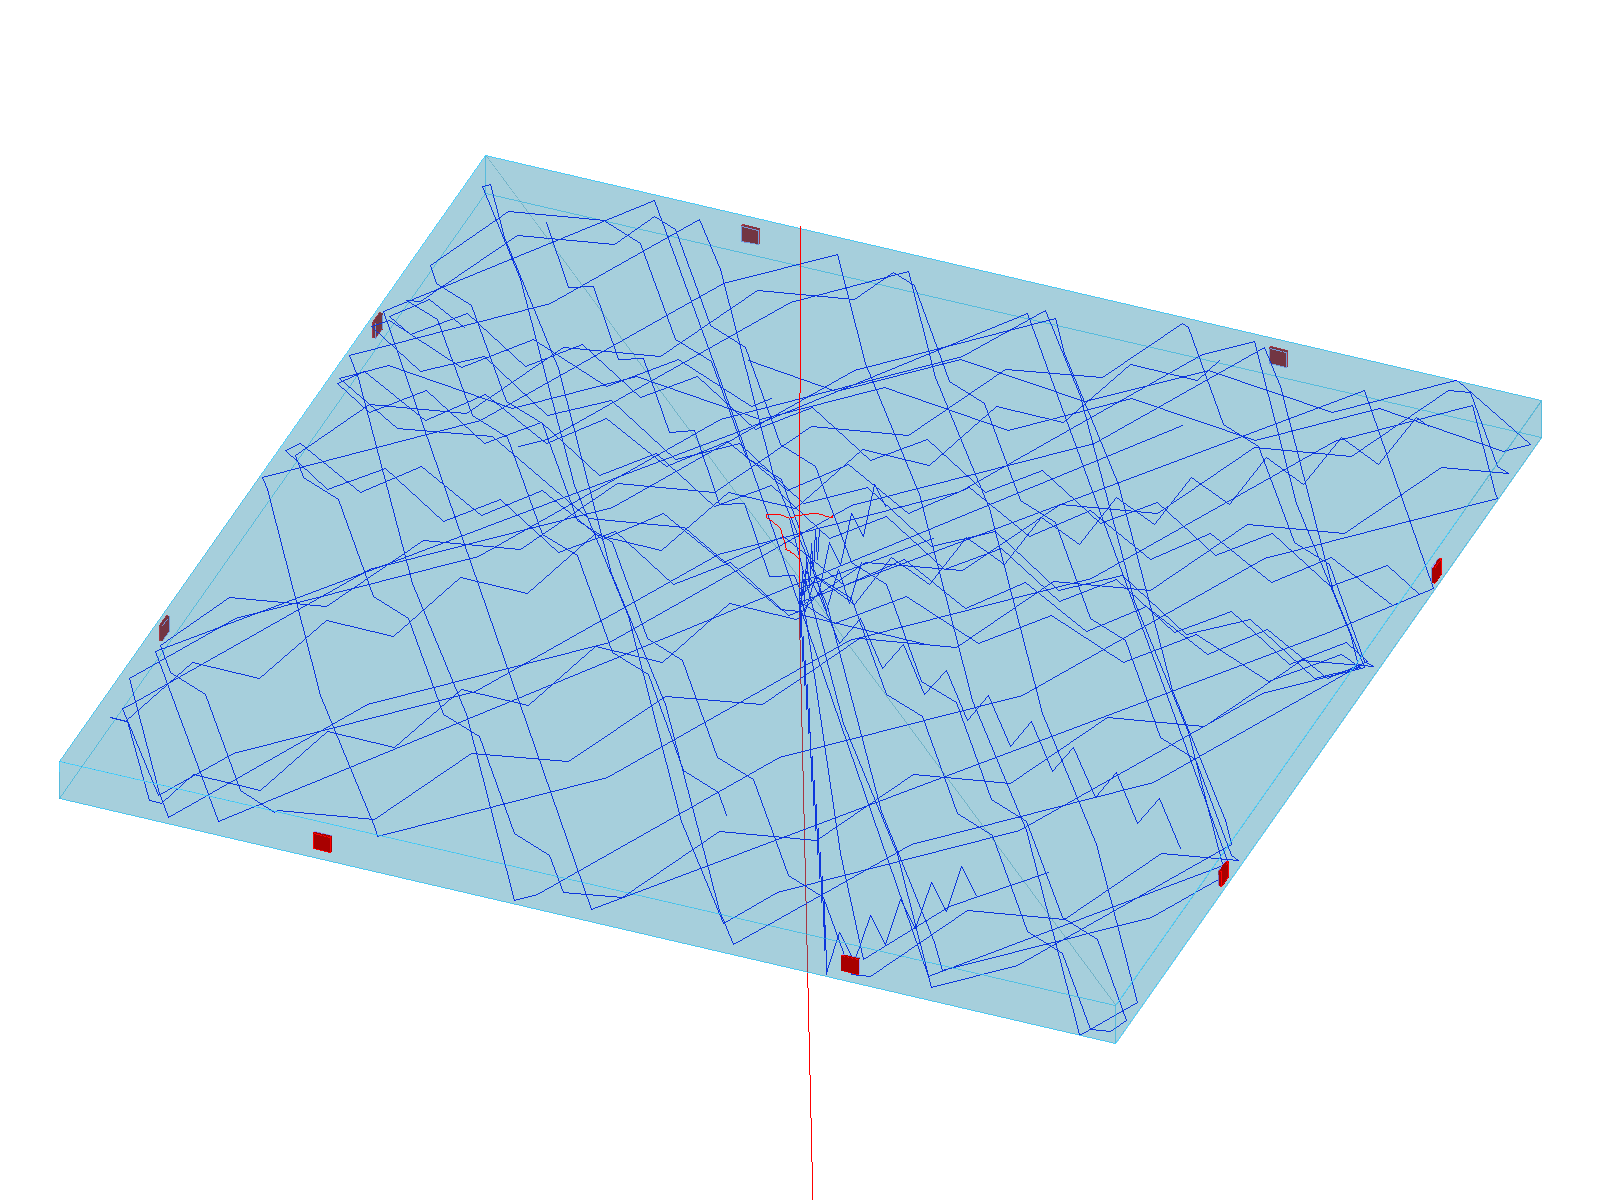
\includegraphics[width=\linewidth]{muon_event_display.png}\\
    {\scriptsize One vertical $\mu$ in glossy plate, cfg-1. Red = muon, blue = optical photons (display only).}
  \end{column}
  \end{columns}
\end{frame}

\begin{frame}{What we compare against Rao}
  \begin{columns}[T]
  \begin{column}{0.58\textwidth}
  \begin{itemize}
    \item Rao reports voltage pulse-height spectra (Fig.~10) for centre / edge / corner ROIs and 4 SiPM configurations.
    \item Our analogue: photoelectrons/event spectra in the same 3 $\times$ 4 grid (\texttt{fig\_pe\_grid}).
    \item Key experimental orderings to test:
    \begin{itemize}
      \item \textbf{Reflectors:} bare $\ll$ TiO$_2$ $<$ Al $\approx$ glossy (glossy/Al best).
      \item \textbf{Position:} corner lowest, centre highest (paper rule).
      \item \textbf{Configs:} cfg-4 (WLS) competitive with direct readout.
    \end{itemize}
    \item Result preview: we reproduce glossy brightest + TiO$_2$ weakest, but \textbf{not} bare-weakest nor corner-lowest everywhere.
  \end{itemize}
  \end{column}
  \begin{column}{0.40\textwidth}
    \centering
    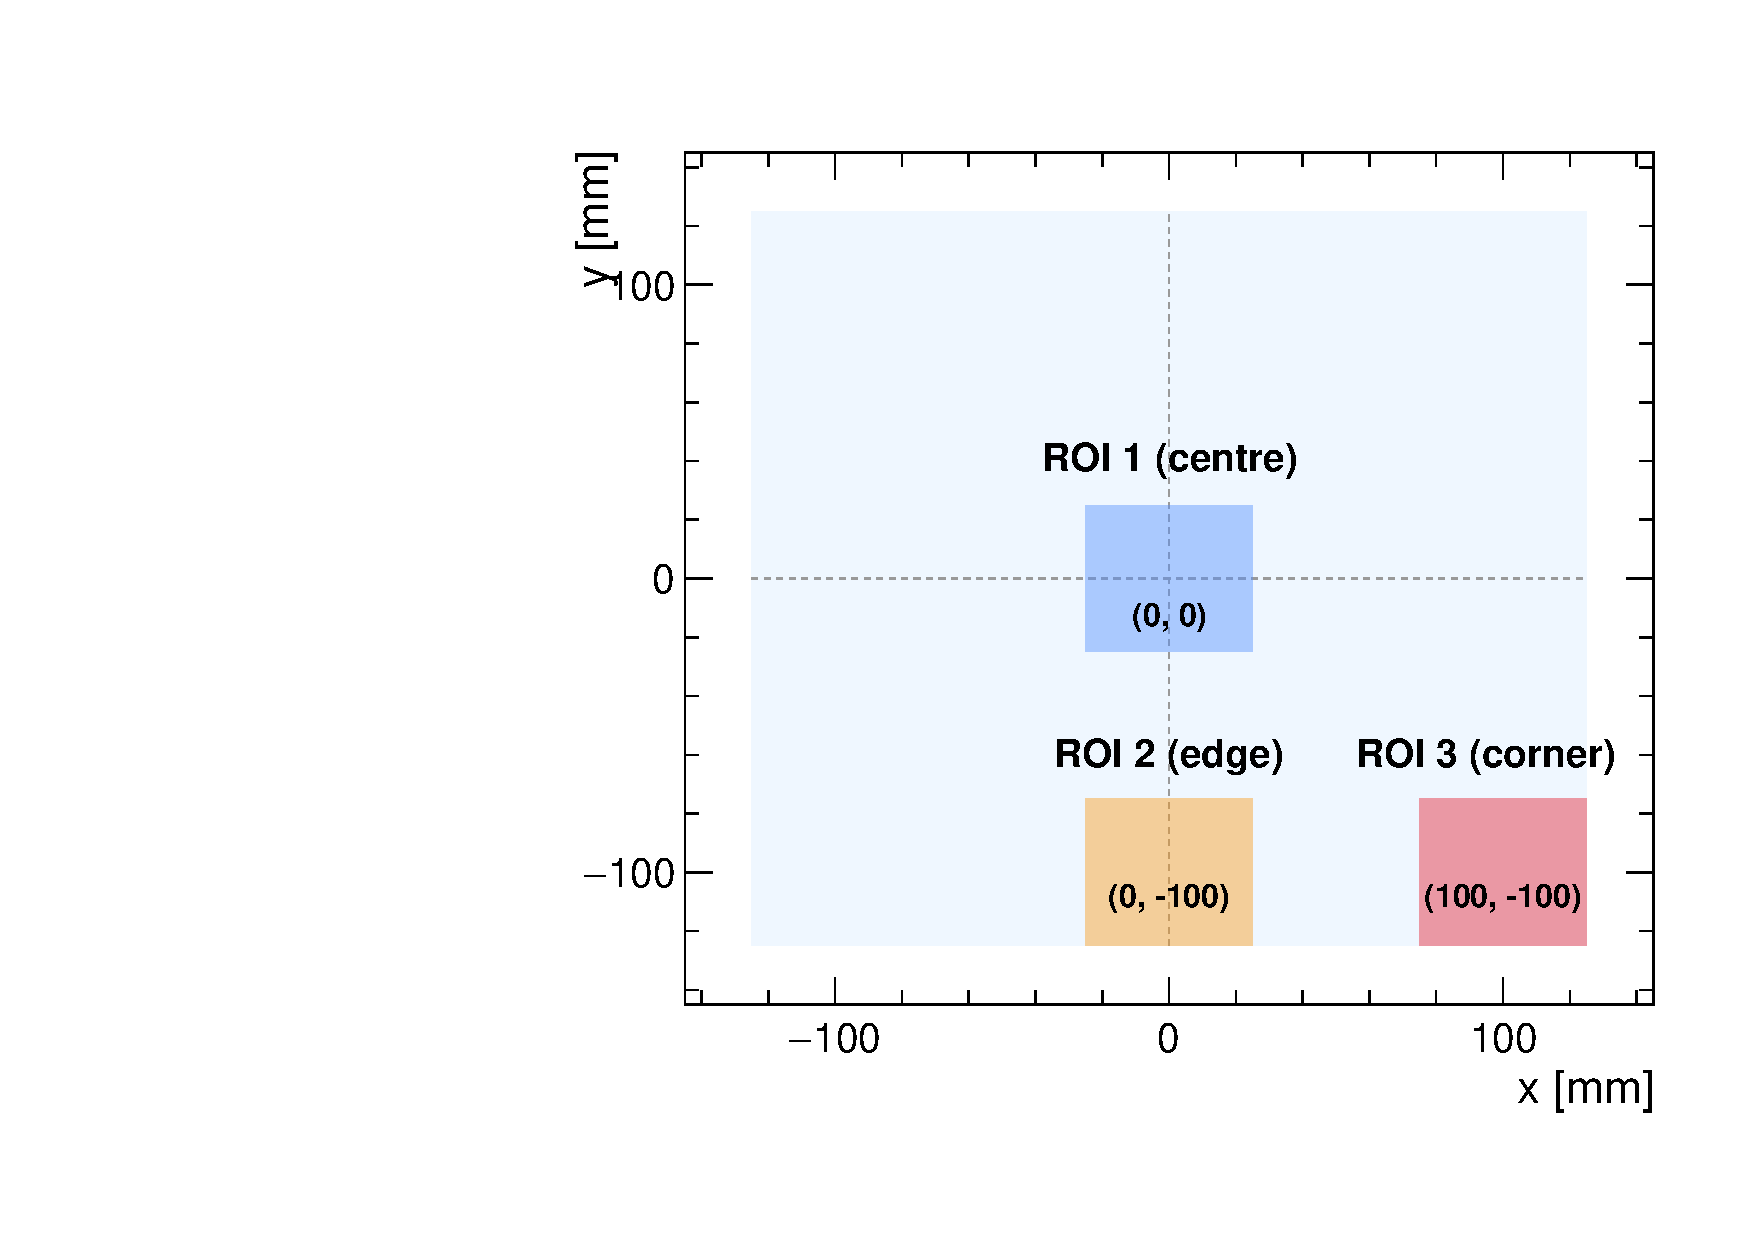
\includegraphics[width=\linewidth]{irradiation_sites.pdf}\\
    {\scriptsize Our three \SI{50}{\milli\meter}$\times$\SI{50}{\milli\meter} ROIs: centre (0,0), edge, corner --- equal area, fully on plate.}
  \end{column}
  \end{columns}
\end{frame}

\section{Simulated detector}

\begin{frame}{Detector layouts (configs 1--4)}
  \begin{columns}[T]
  \begin{column}{0.52\textwidth}
  \begin{itemize}
    \item Plate: PVT \SI{250}{\milli\meter}$\times$\SI{250}{\milli\meter}$\times$\SI{10}{\milli\meter}, $n=1.58$, polished, EJ-200/UPS-923A tables.
    \item SiPM: $4\times4$~\si{\milli\meter} epoxy box ($n=1.55$) + \SI{0.1}{\milli\meter} grease pad ($n=1.46$).
    \item \textbf{Cfg-1:} 8 SiPMs, 2 per side at $\pm 50$\% half-length.
    \item \textbf{Cfg-2:} 4 SiPMs, 1 per side at same offsets (C4-symmetric).
    \item \textbf{Cfg-3:} 2 SiPMs, both on $-x$ face (report top edge).
    \item \textbf{Cfg-4:} 1 SiPM + WLS fibre clamp on $-x$ face (next slide).
  \end{itemize}
  \end{column}
  \begin{column}{0.46\textwidth}
    \centering
    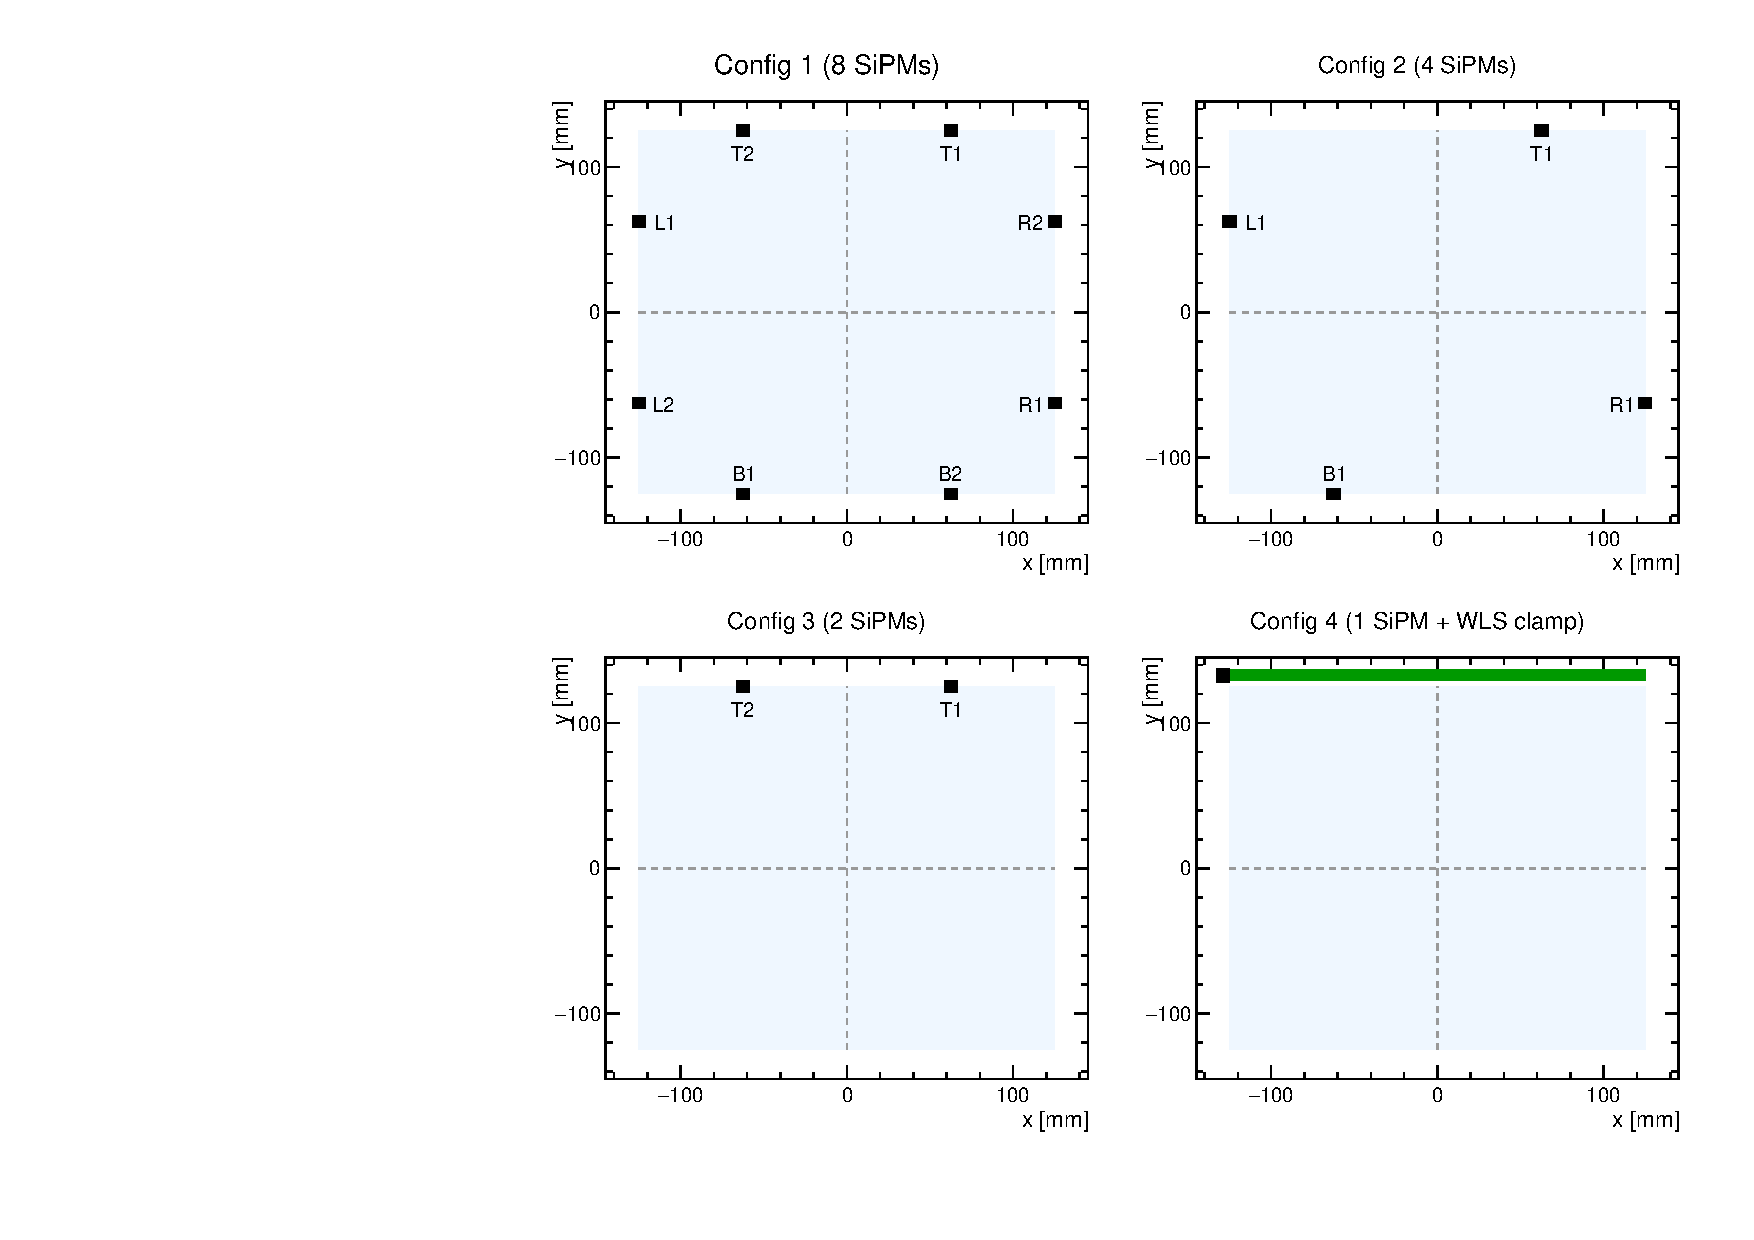
\includegraphics[width=\linewidth]{sipm_layouts.pdf}\\
    {\scriptsize Schematics: black squares = SiPMs; green bar = cfg-4 clamp + readout SiPM at top-left.}
  \end{column}
  \end{columns}
\end{frame}

\begin{frame}{Reflector treatments: the heart of the model}
  \centering
  {\footnotesize
  \begin{tabular}{lllll}
    \toprule
     & \textbf{Bare} & \textbf{TiO$_2$} & \textbf{Al foil} & \textbf{Glossy} \\
    \midrule
    Contact & \SI{1.2}{\milli\meter} air gap & direct & grease / air & air gap \\
    G4 finish & none (Fresnel/TIR) & groundfrontpainted & polishedbackpainted & polishedbackpainted \\
    $R(\lambda)$ & --- (TIR guide) & 0.955--0.983 & 0.904--0.925 & 0.900--0.955 \\
    Character & lossless guide & Lambertian, no TIR & specular, TIR + mirror & lossier mirror \\
    \bottomrule
  \end{tabular}}
  \vspace{0.4em}

  \begin{columns}[T]
  \begin{column}{0.55\textwidth}
    \centering
    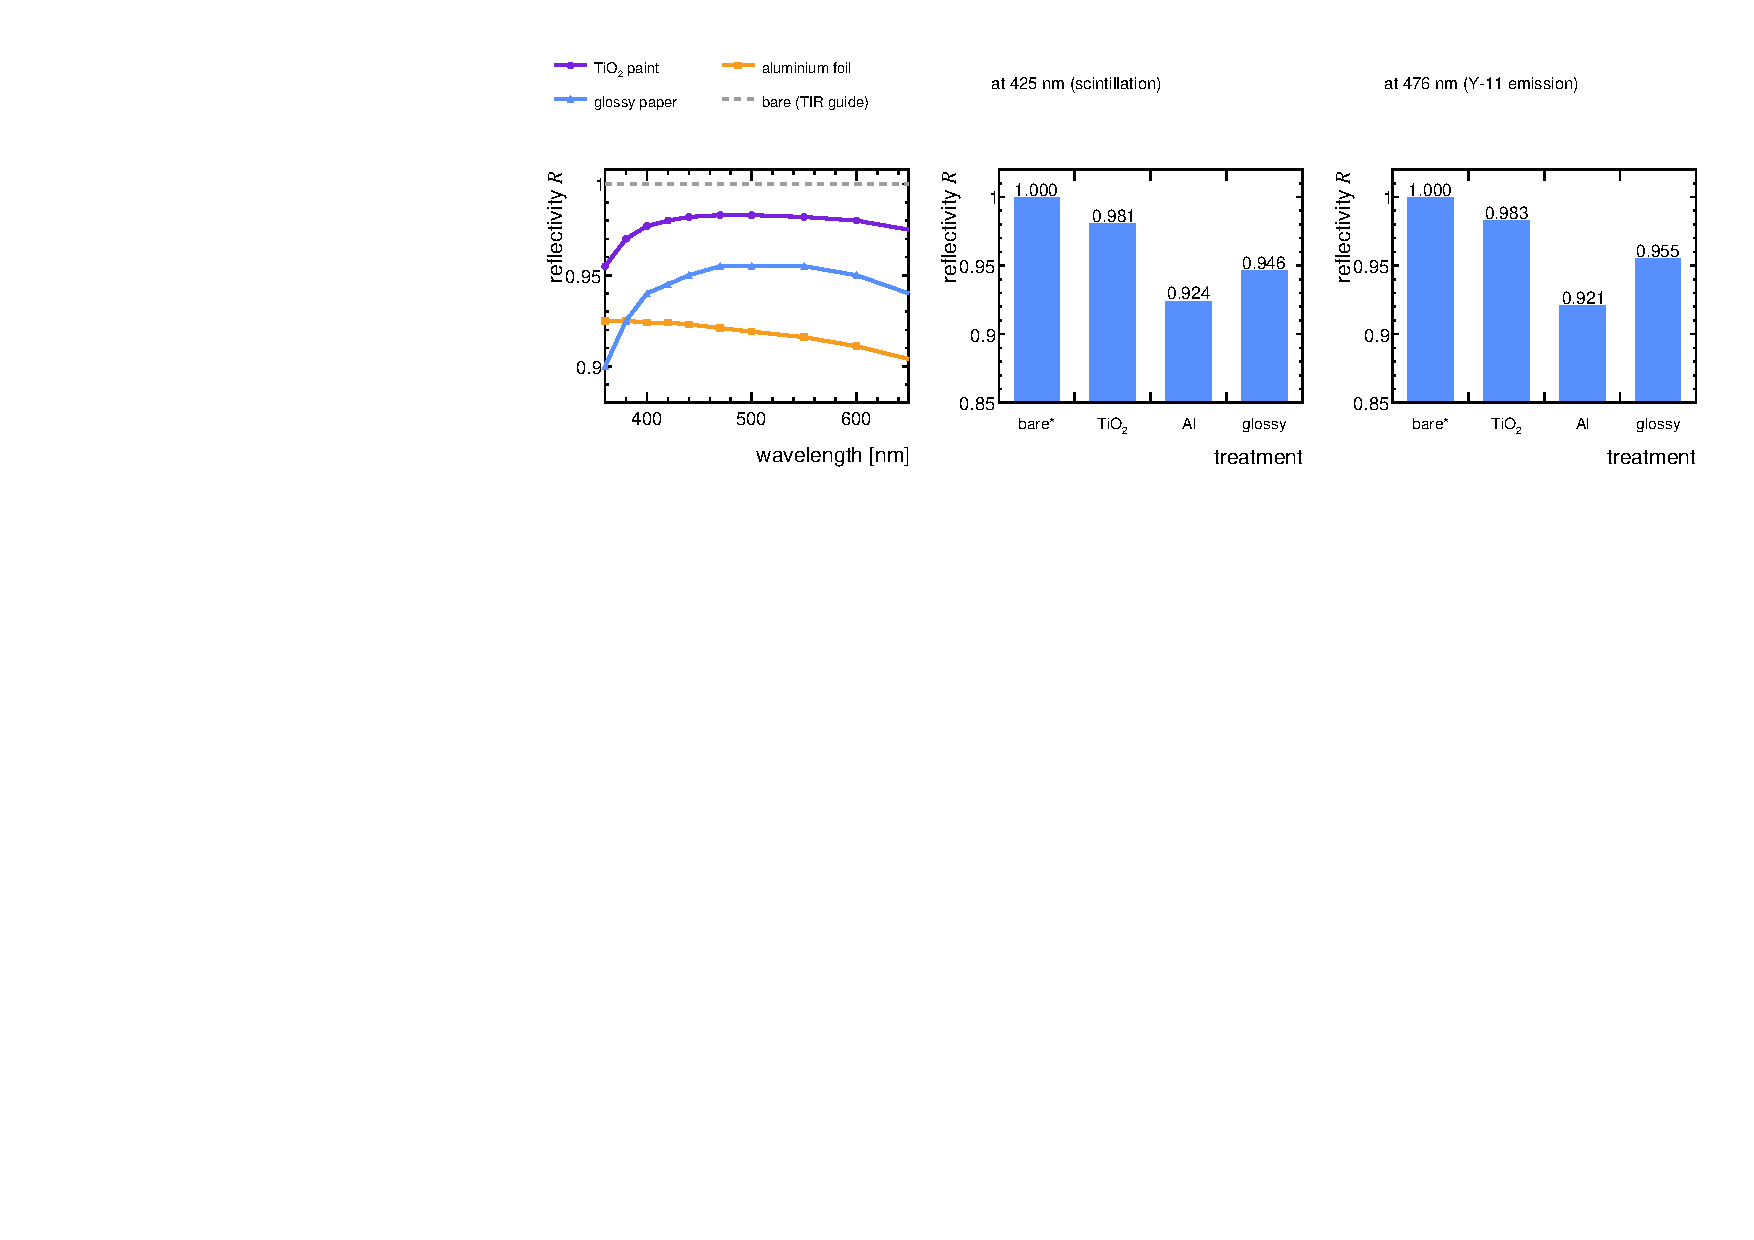
\includegraphics[width=\linewidth]{reflector_reflectivity.pdf}
  \end{column}
  \begin{column}{0.43\textwidth}
    {\small
    \begin{itemize}
      \item Bare: no skin; sub-critical light killed in black holder ($R=T=0$ skin + \SI{1}{\micro\meter} bulk).
      \item Optional bare-contact fraction $f$ ($R=1-f$): frustrated-TIR bracket.
      \item Al backing switch: \texttt{grease} ($n=1.46$) vs \texttt{air} ($n=1.0003$) --- changes $\theta_c$, not $R$.
    \end{itemize}}
  \end{column}
  \end{columns}
\end{frame}

\section{Optical inputs and SiPM model}

\begin{frame}{Spectral inputs actually fed to Geant4}
  \begin{center}
    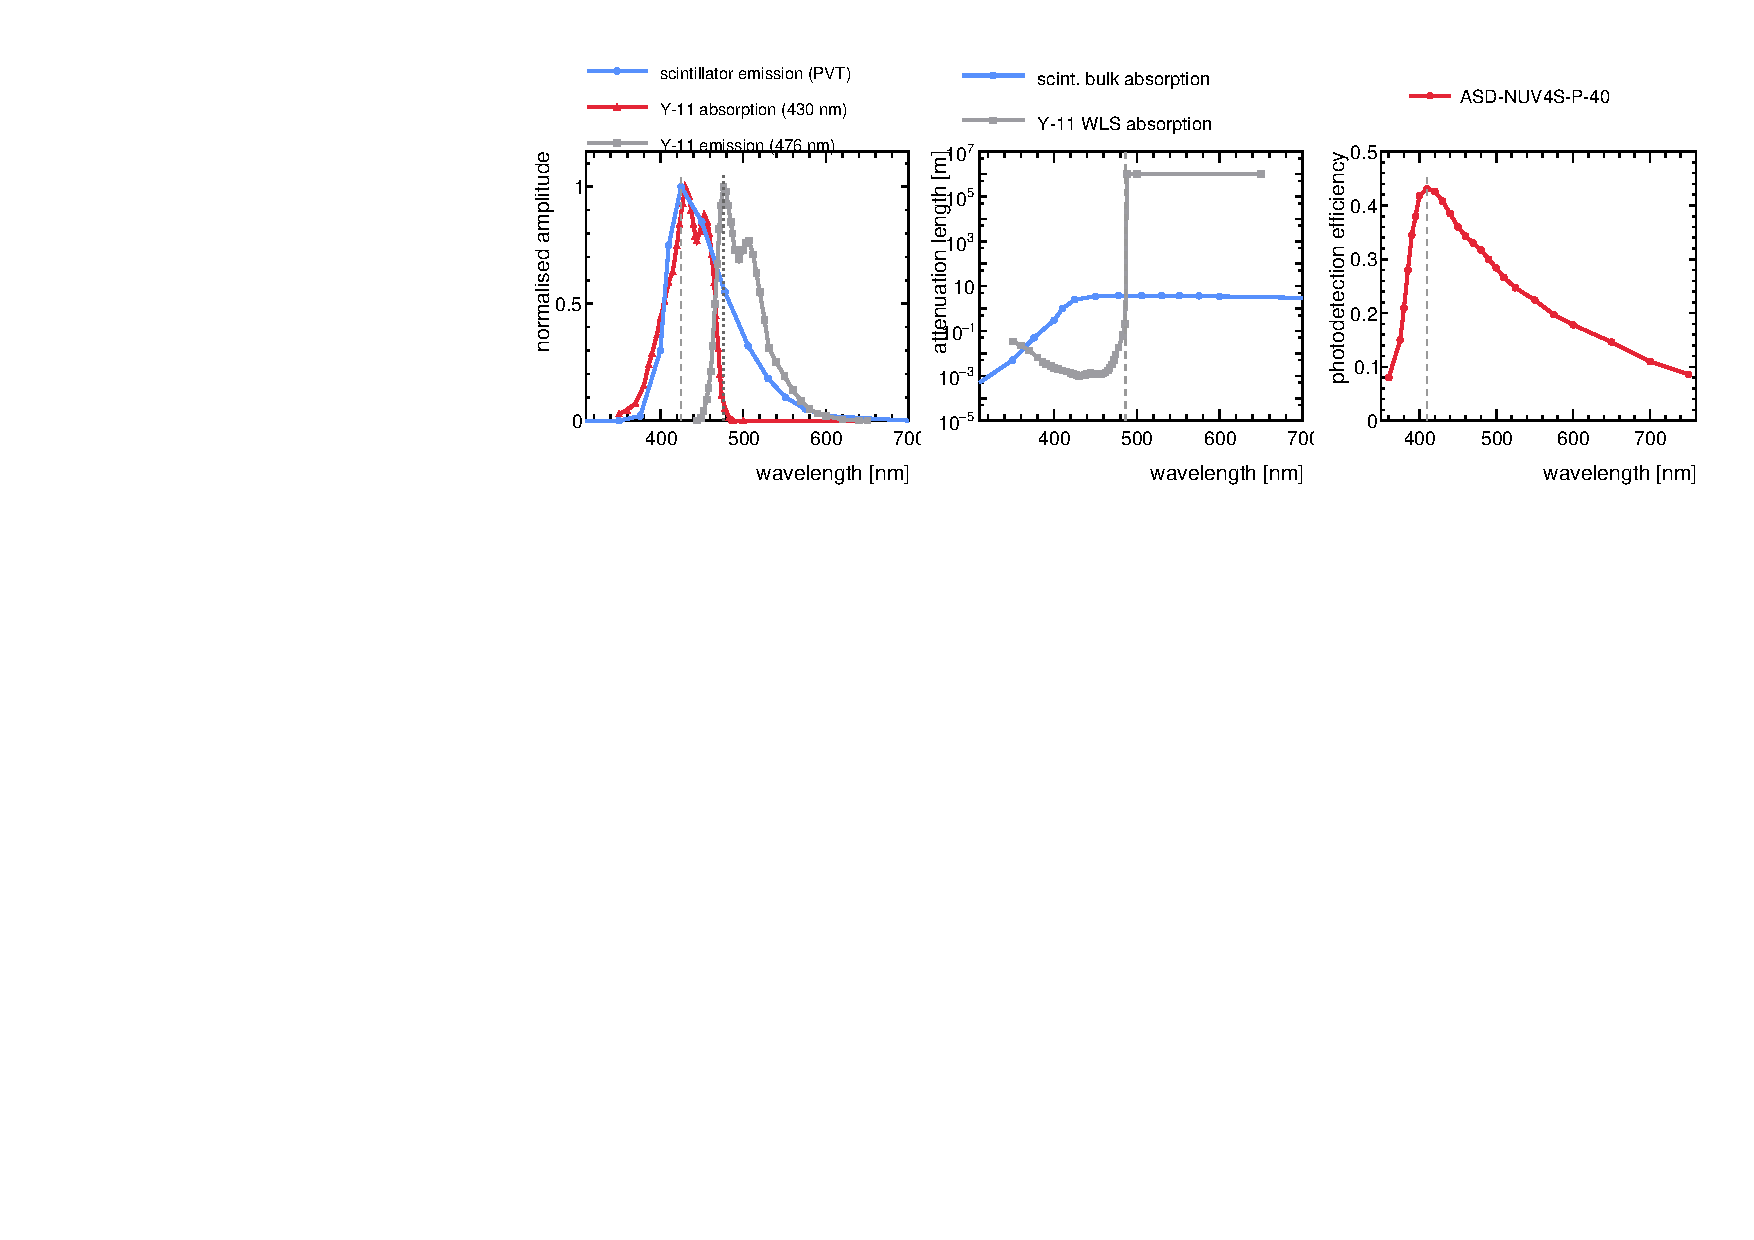
\includegraphics[width=0.92\linewidth]{optical_spectra.pdf}
  \end{center}
  {\small Left: scintillator emission (\SI{425}{\nano\meter}), Y-11 absorption (\SI{430}{\nano\meter}) + re-emission (\SI{476}{\nano\meter}). Middle: bulk vs WLS attenuation (WLS $L=\SI{1.0}{\milli\meter}$ at \SI{430}{\nano\meter}). Right: ASD-NUV4S-P-40 PDE, peak 0.431 at \SI{410}{\nano\meter}. All digitized tables, linearly interpolated.}
\end{frame}

\begin{frame}{Timing, index ladder, and SiPM detection}
  \begin{columns}[T]
  \begin{column}{0.55\textwidth}
    \centering
    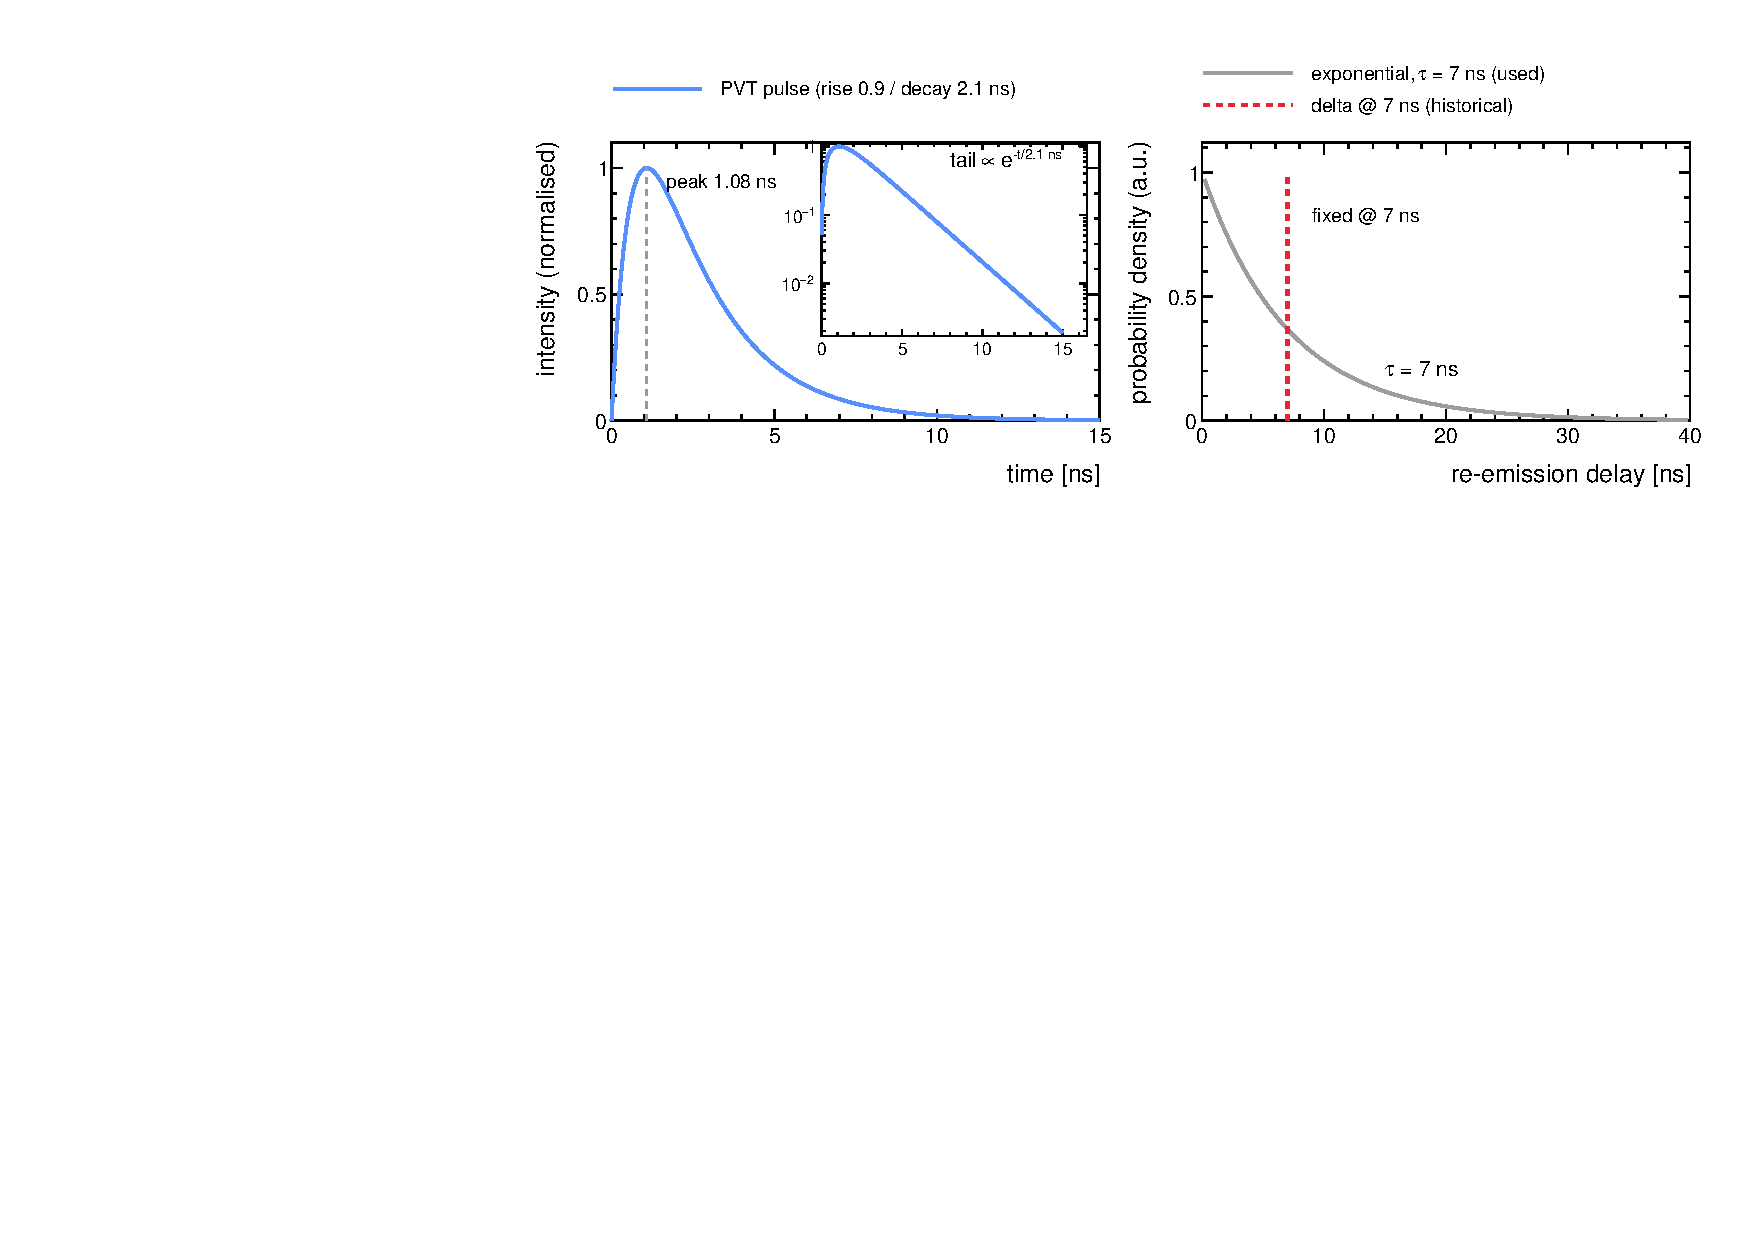
\includegraphics[width=\linewidth]{optical_timing.pdf}\\
    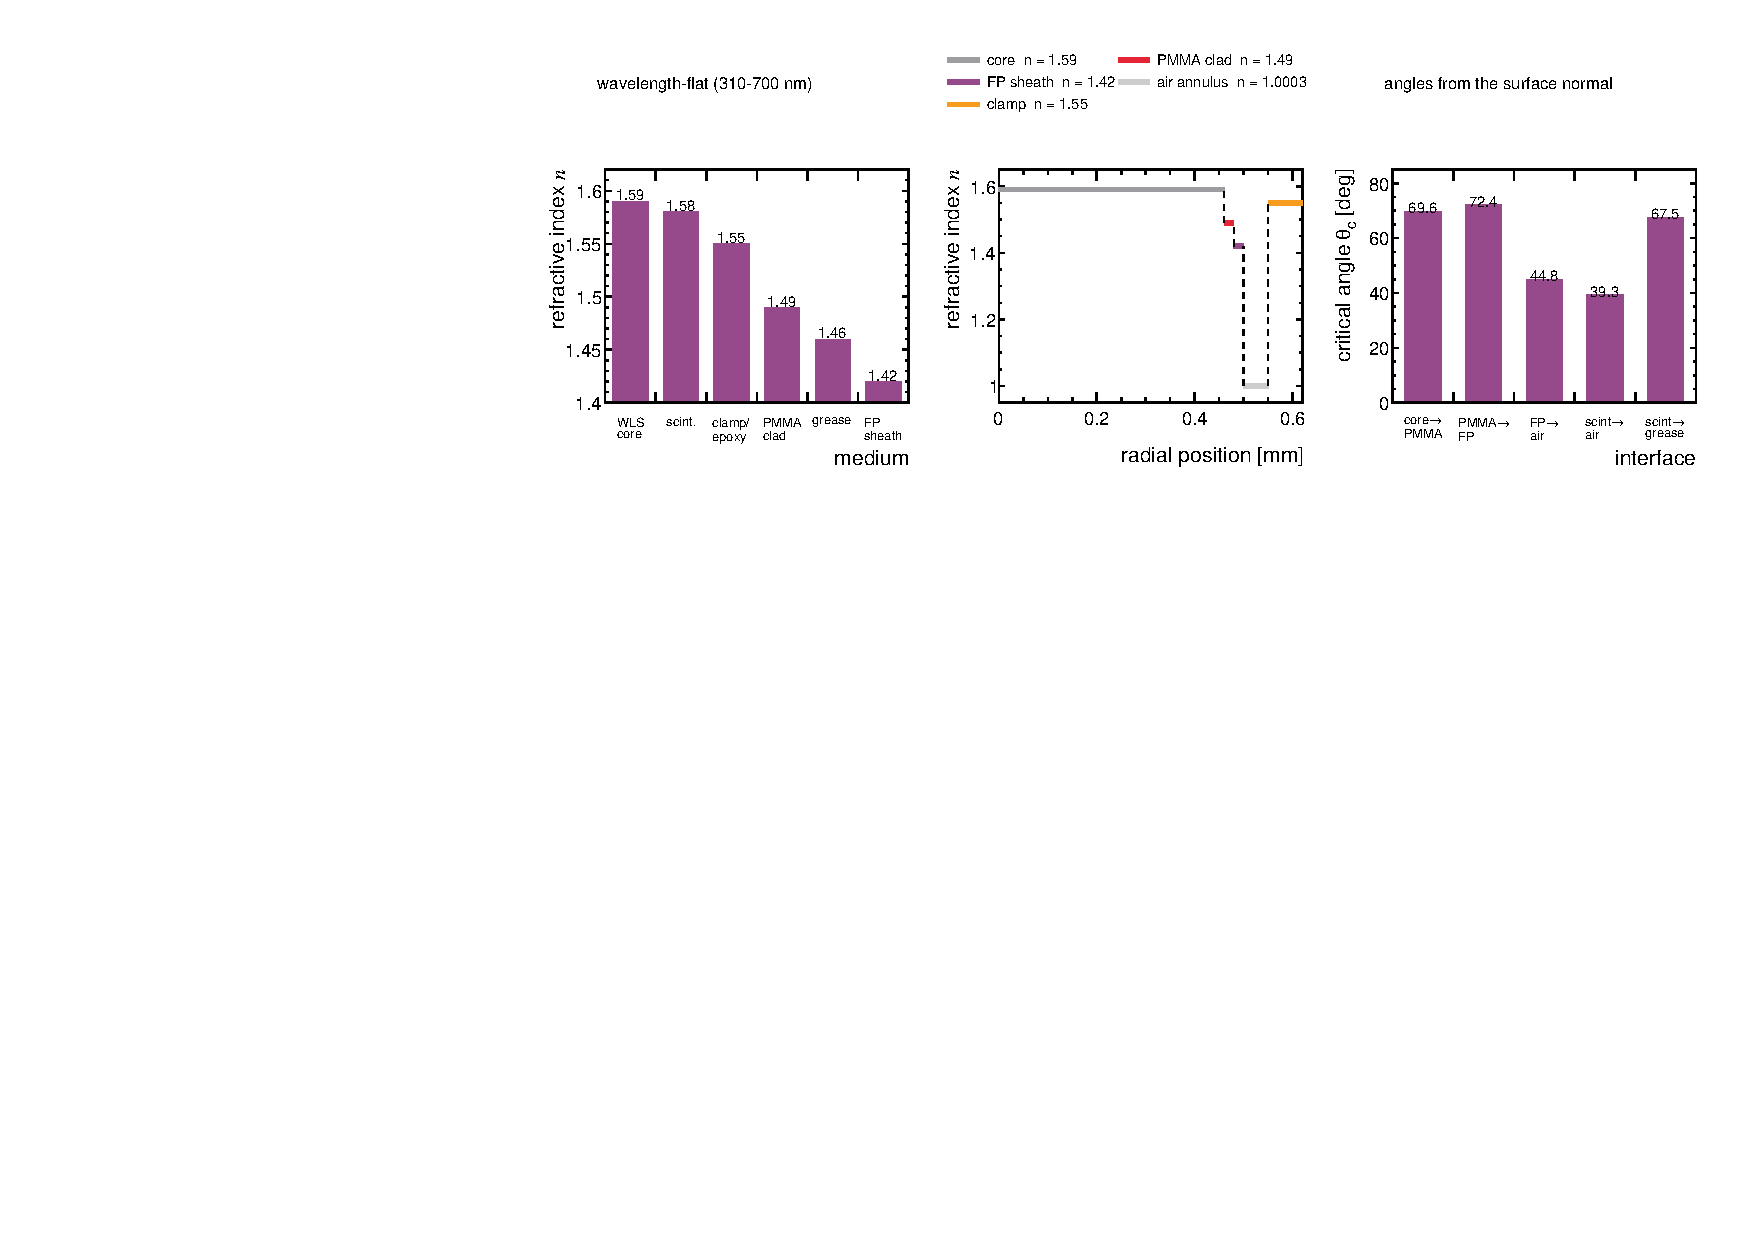
\includegraphics[width=\linewidth]{refractive_index.pdf}
  \end{column}
  \begin{column}{0.43\textwidth}
    {\small
    \begin{itemize}
      \item Scintillation: $f(t)\propto(1-e^{-t/0.9})e^{-t/2.1}$~ns, peak at \SI{1.08}{\nano\meter}; WLS re-emission exponential $\tau=\SI{7}{\nano\meter}$ (not fixed delay).
      \item Fibre staircase $1.59/1.49/1.42$ + air annulus sustains core--cladding TIR.
      \item SiPM = \texttt{dielectric\_metal} border with \texttt{EFFICIENCY} = PDE$(\lambda)$, $R=0$; \texttt{G4OpBoundaryProcess} draws PDE, sets \texttt{Detection}, invokes SD --- no manual draw; SD counts 1~pe per hit.
      \item Per-event accounting: $N_\gamma$ produced vs $N_{\rm pe}$ detected; \texttt{sipmHits} rows carry $t_{\rm first}$, $\langle\lambda\rangle$, per-pe $t$/$\lambda$/creator vectors.
    \end{itemize}}
  \end{column}
  \end{columns}
\end{frame}

\section{Config 4: WLS fibre clamp}

\begin{frame}{Config 4 close-up: analytic multi-clad Y-11 bundle}
  \begin{columns}[T]
  \begin{column}{0.50\textwidth}
    {\small
    \begin{itemize}
      \item 4 $\times$ \O\SI{1.0}{\milli\meter} Kuraray Y-11(200) fibres, full \SI{250}{\milli\meter} along $-x$ face.
      \item \SI{2.5}{\milli\meter} pitch $\to$ \SI{1.0}{\milli\meter} touching bundle over \SI{41}{\milli\meter} convergence; analytic mitered \texttt{G4CutTubs} legs (no stuck tracks).
      \item Core $n=1.59$ / PMMA $1.49$ / sheath $1.42$; \SI{0.05}{\milli\meter} air annulus in \O\SI{1.1}{\milli\meter} channels (deliberate!).
      \item \SI{0.10}{\milli\meter} grease film; white Lambertian clamp ($R=0.85$) on all faces; far-end Al mirror caps with explicit skin (fixes silent \texttt{NoRINDEX} kill, +40\% centre).
      \item WLS: digitized Y-11 absorption + emission, $E'_\gamma \le E_\gamma$; $\tau=\SI{7}{\nano\meter}$ exponential.
    \end{itemize}}
  \end{column}
  \begin{column}{0.48\textwidth}
    \centering
    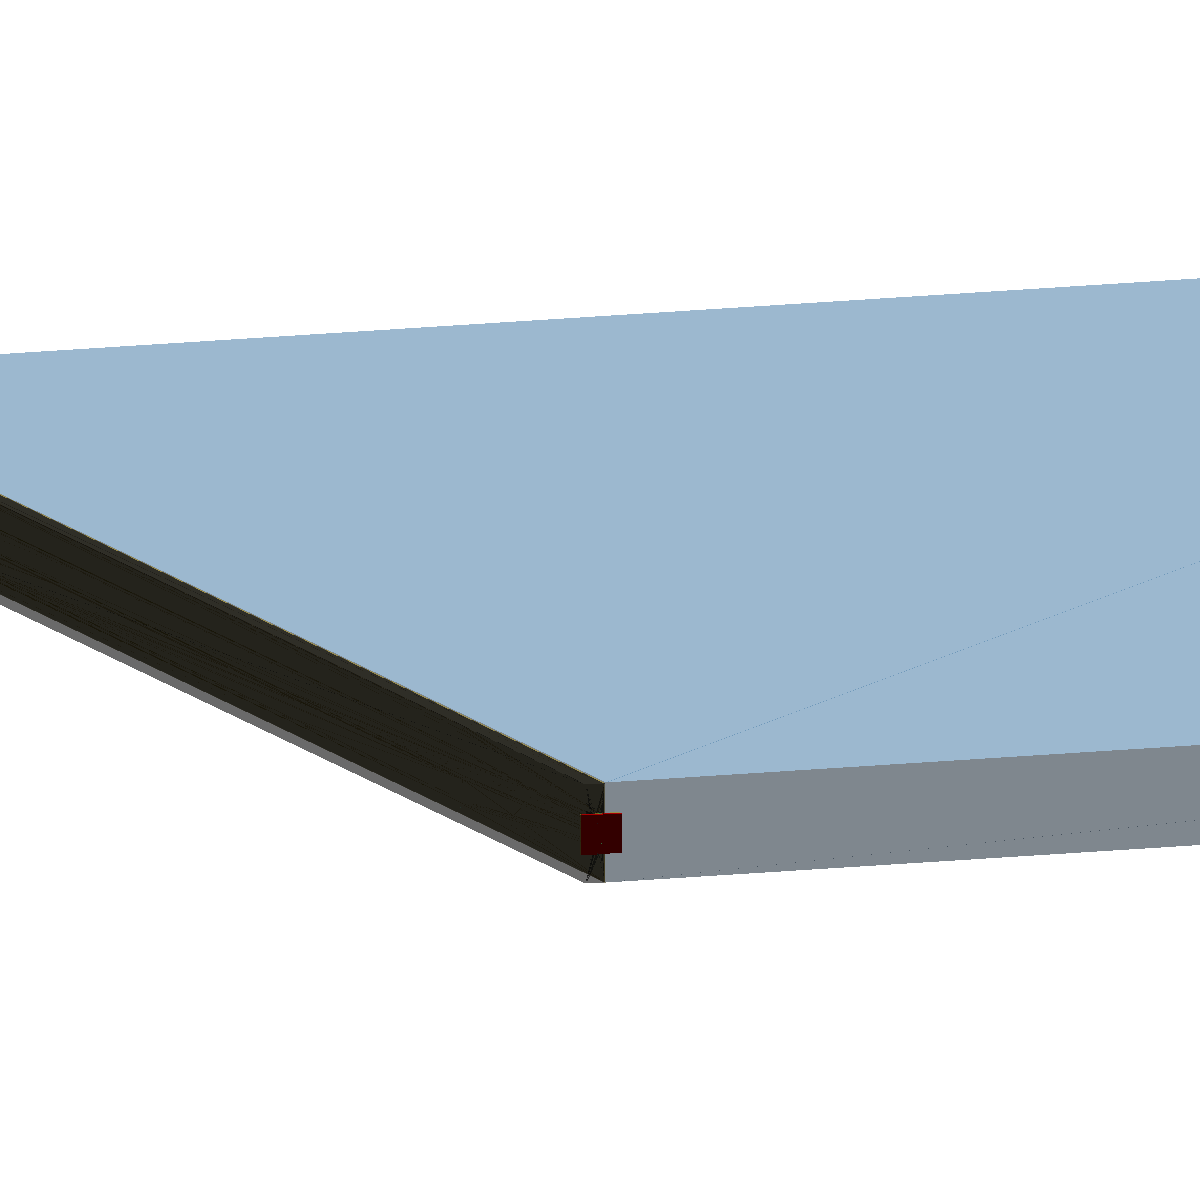
\includegraphics[width=0.85\linewidth]{wls_ogl_overview.png}\\
    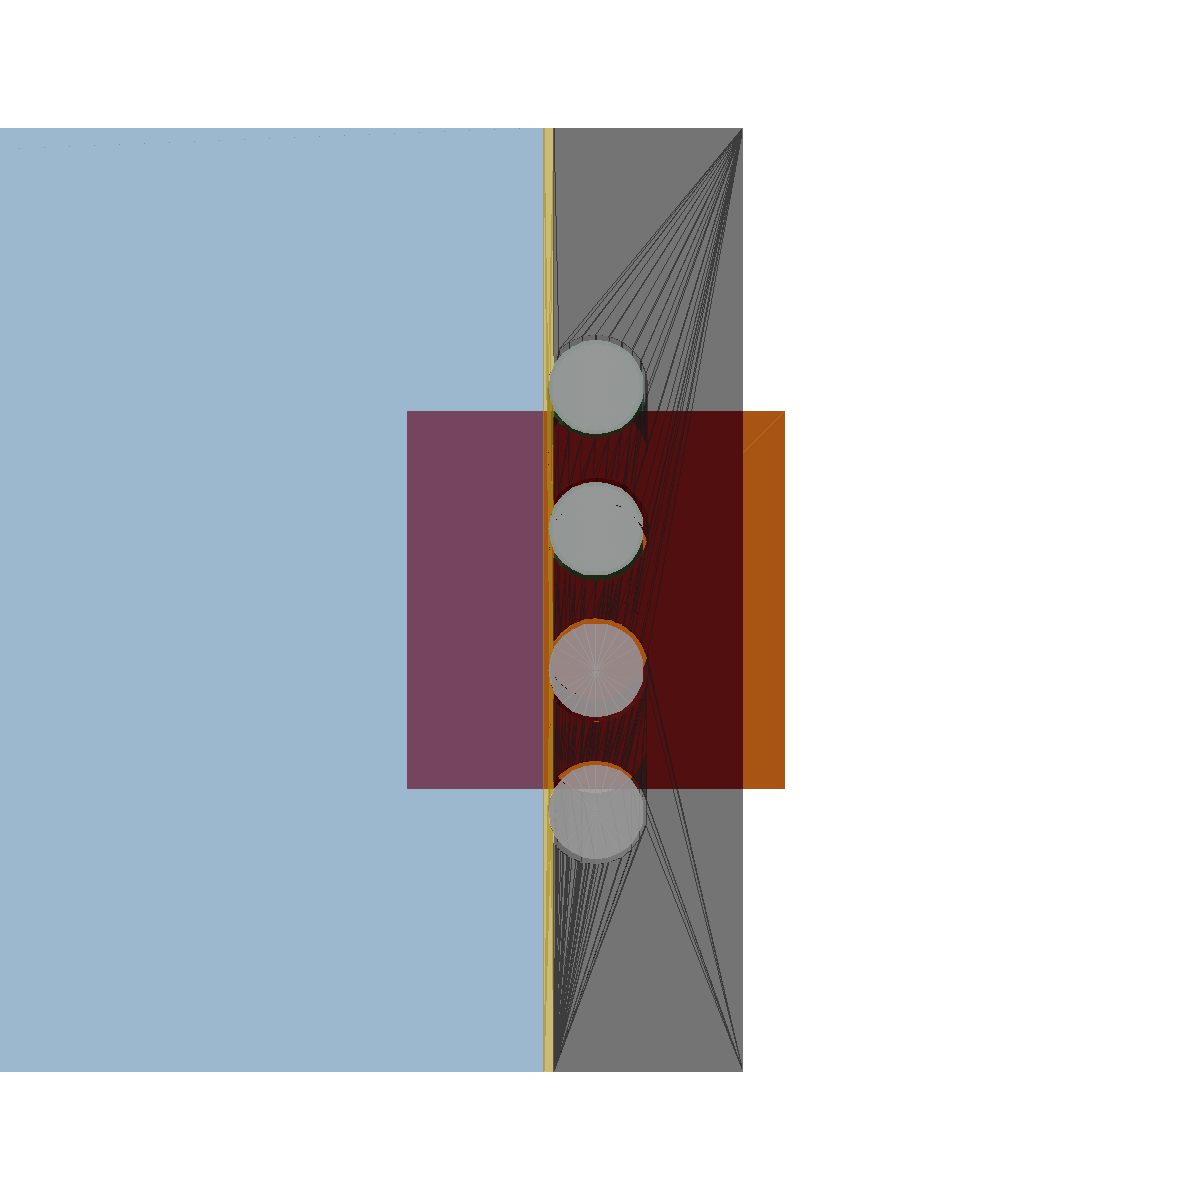
\includegraphics[width=0.47\linewidth]{wls_ogl_xsection.png}\hfill
    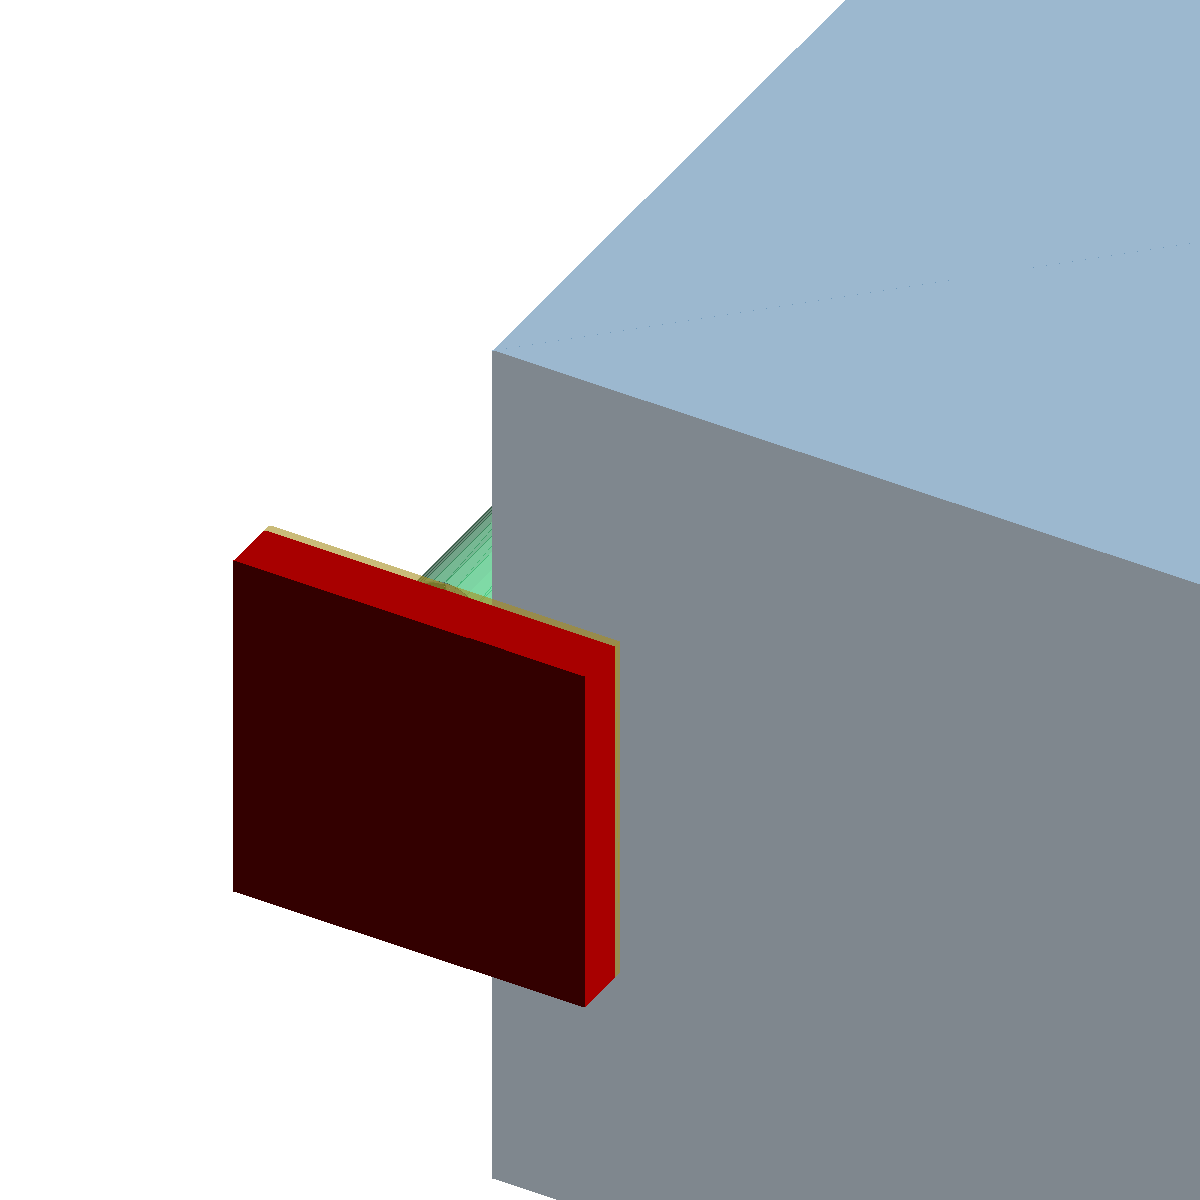
\includegraphics[width=0.47\linewidth]{wls_ogl_coupling.png}\\
    {\scriptsize Overview / cross-section / bundle-to-SiPM coupling (Boolean clamp hidden in right panel).}
  \end{column}
  \end{columns}
\end{frame}

\section{Results}

\begin{frame}{WLS works: detected spectrum green-shifts by \SI{52}{\nano\meter}}
  \begin{center}
    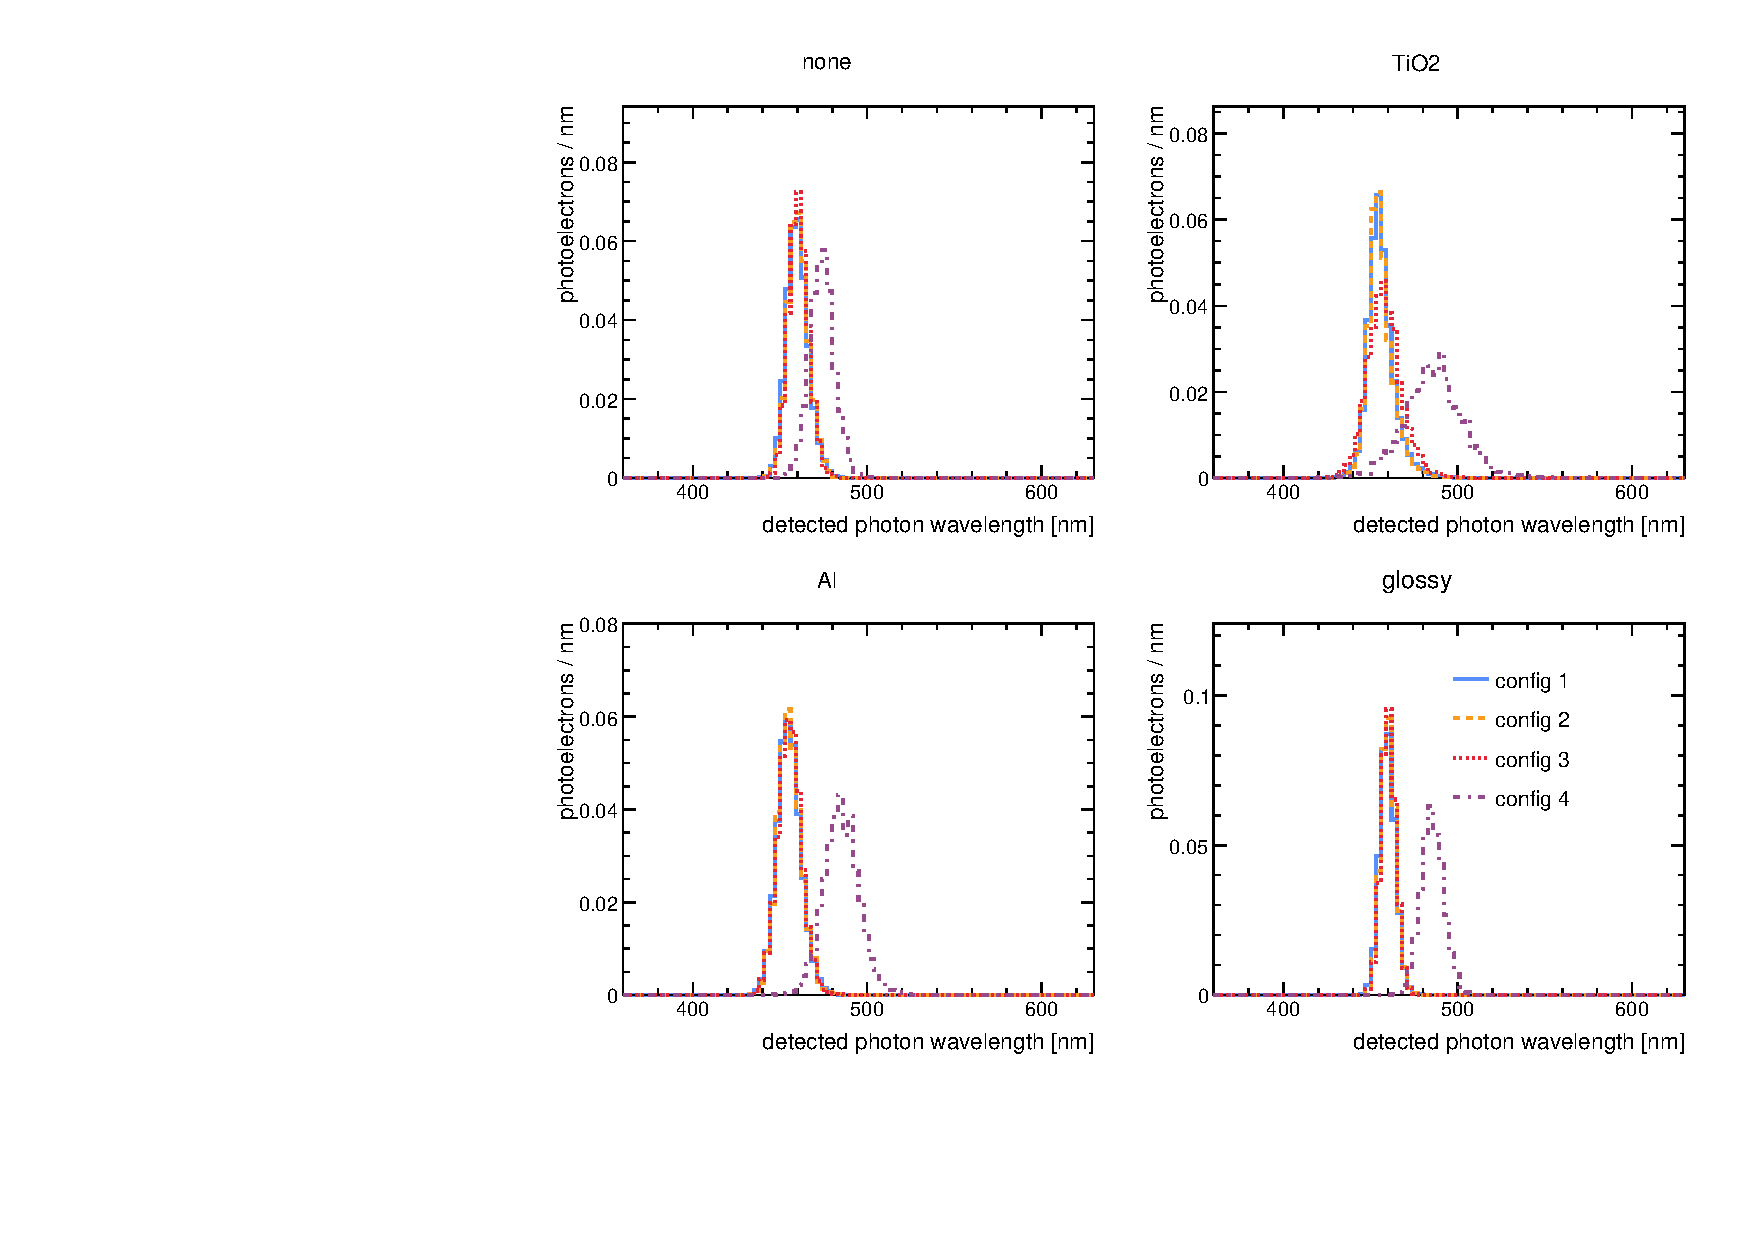
\includegraphics[width=0.85\linewidth]{fig_wavelength_cfg.pdf}
  \end{center}
  {\small Cfgs~1--3: identical blue scintillation ($\approx$\SI{457}{\nano\meter}, red-shifted from 425 by self-absorption). Cfg-4: \SI{509.5}{\nano\meter} green via Y-11 --- same shift for every wrapper, so it comes from the fibre, not the wrapper. Cf.\ report Fig.~12.}
\end{frame}

\begin{frame}{Photoelectron spectra: Rao Fig.~10 analogue}
  \begin{center}
    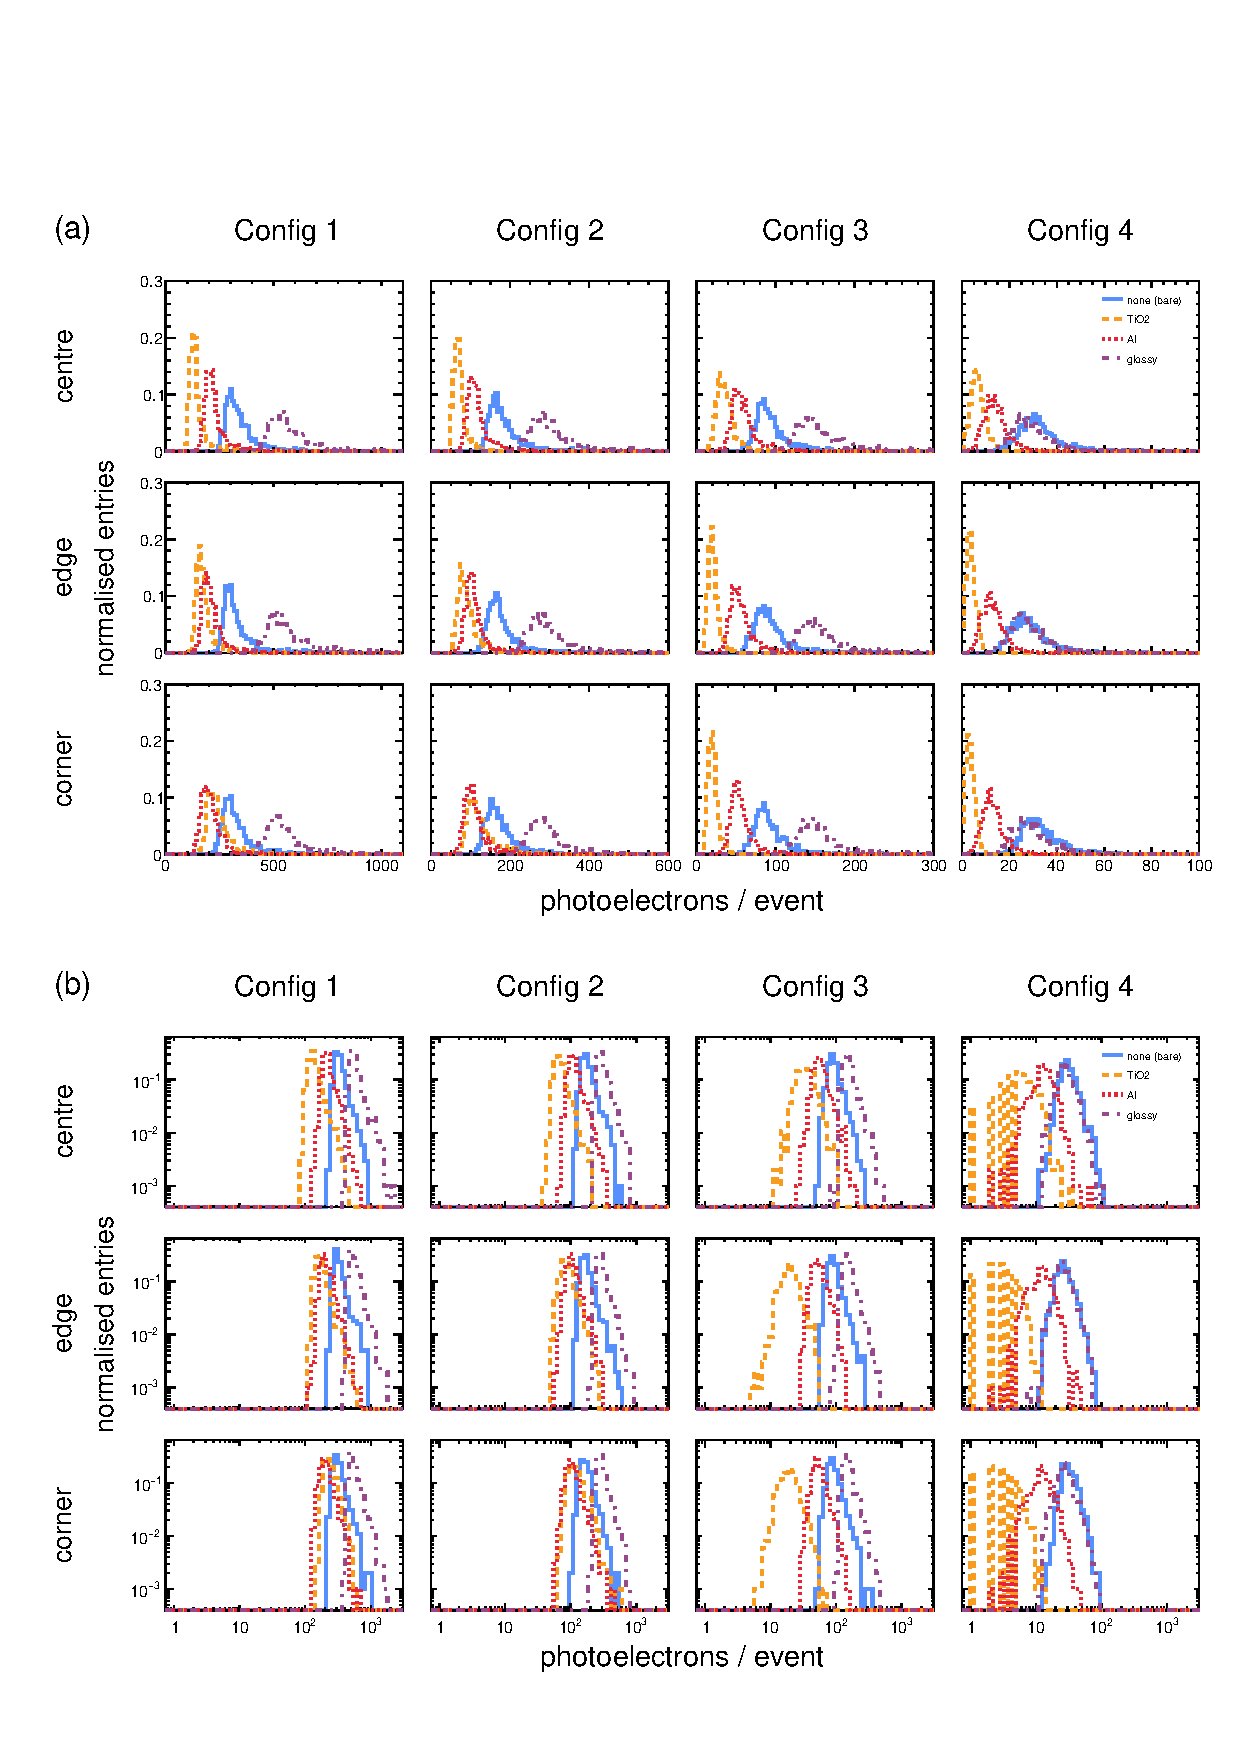
\includegraphics[height=0.78\textheight,keepaspectratio]{fig_pe_grid.pdf}
  \end{center}
  {\small Rows = centre/edge/corner, columns = cfg~1--4, colours = wrappers. Ordering TiO$_2$ $<$ Al $<$ bare $<$ glossy in every direct-coupled cell (cfg-1 centre: 125 / 200 / 304 / 521~pe). Cfg-4 an order of magnitude dimmer. TiO$_2$ varies $\sim$1.75$\times$ by position; others $\le$9\%.}
\end{frame}

\begin{frame}{Plate-averaged efficiency (whole-slab, 25k events/cell)}
  \begin{columns}[T]
  \begin{column}{0.58\textwidth}
    \centering
    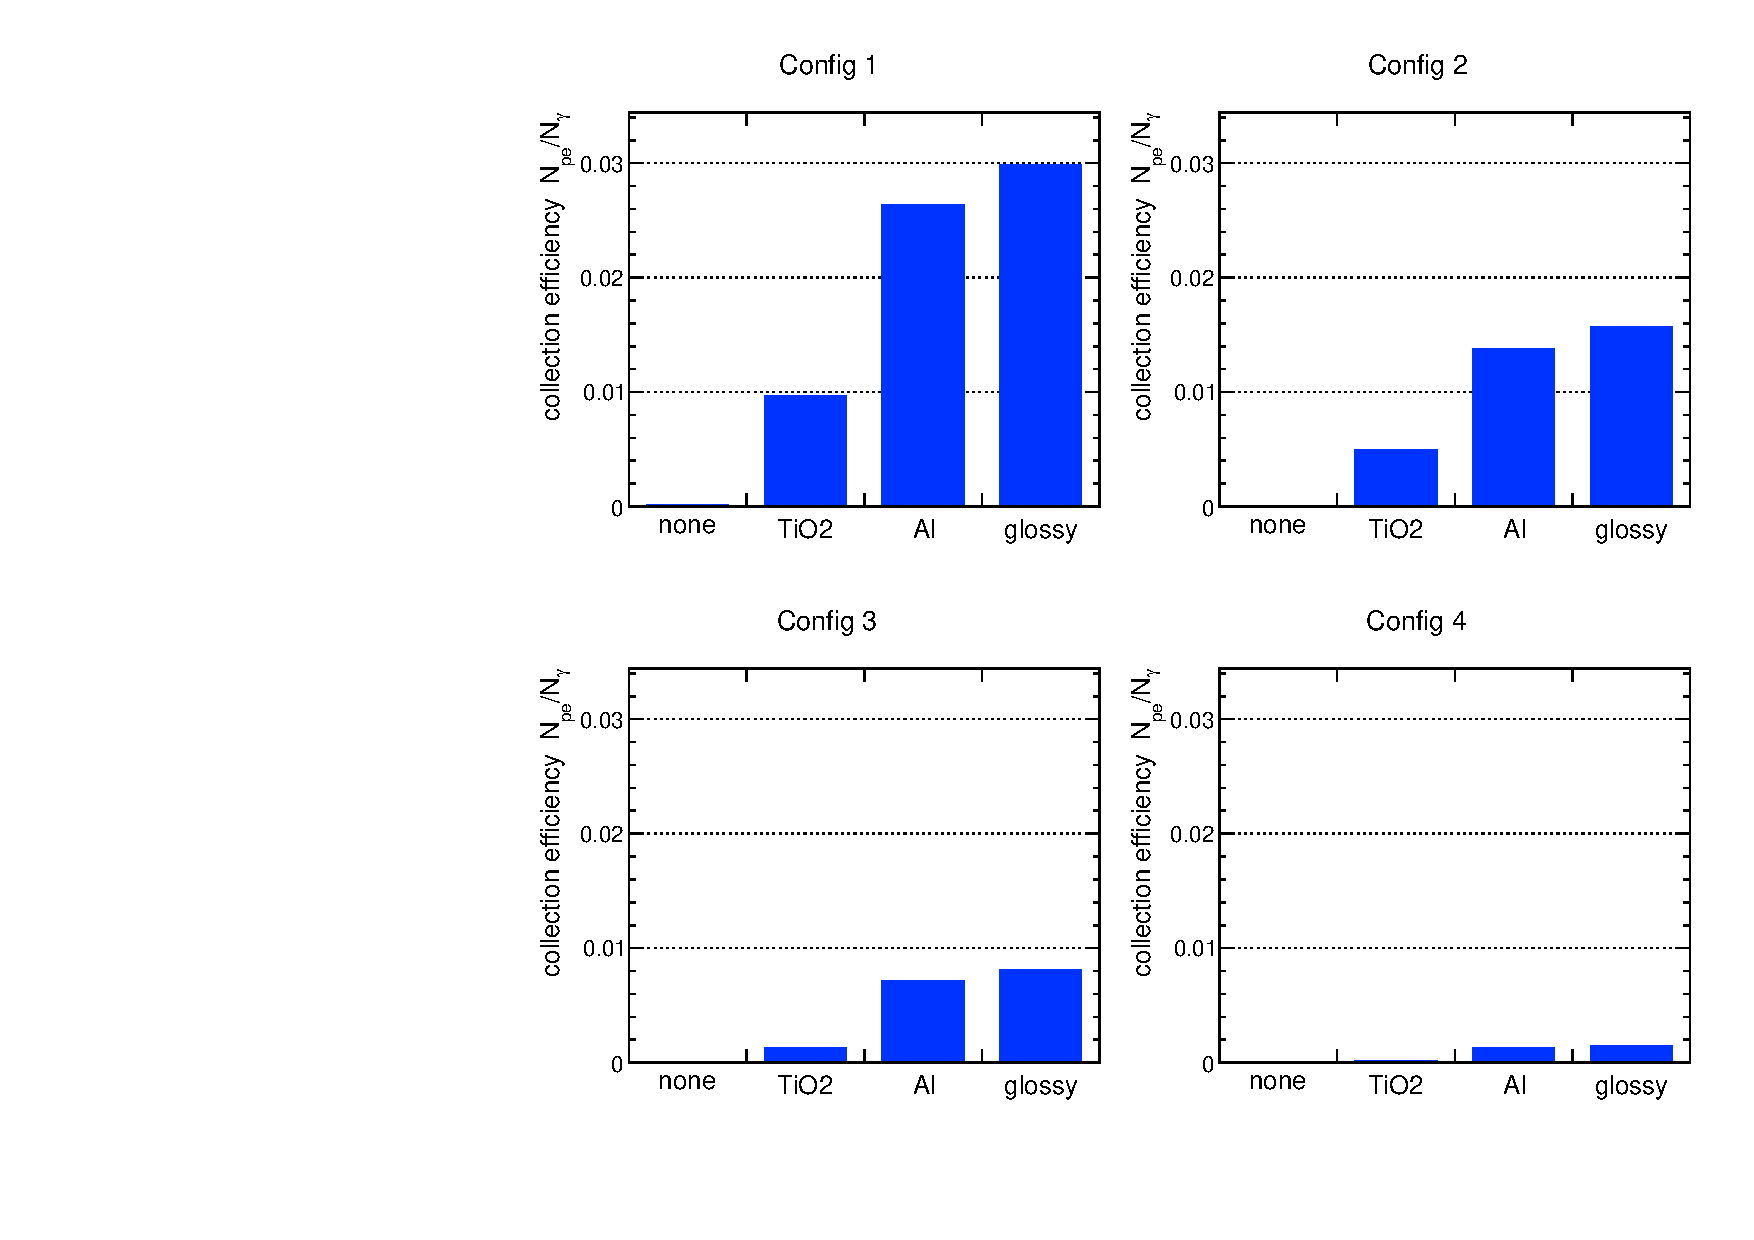
\includegraphics[width=\linewidth]{fig_eff_bars.pdf}\\
    {\scriptsize $\varepsilon=\sum N_{\rm pe}/\sum N_\gamma$. Glossy brightest everywhere; bare second, not weakest.}
  \end{column}
  \begin{column}{0.40\textwidth}
    {\small
    \begin{tabular}{lcccc}
      \toprule
       & Bare & TiO$_2$ & Al & Glossy \\
      \midrule
      Cfg-1 & 1.56 & 0.95 & 1.05 & 2.65 \\
      Cfg-2 & 0.82 & 0.48 & 0.54 & 1.40 \\
      Cfg-3 & 0.42 & 0.24 & 0.27 & 0.71 \\
      Cfg-4 & 0.17 & 0.16 & 0.15 & 0.35 \\
      \bottomrule
    \end{tabular}\\
    {\scriptsize $\varepsilon\times10^{-2}$. Scales $\approx$ with sensor area; cfg-4 $\approx$1.5--2.5$\times$ below cfg-3. Cf.\ report Fig.~16 discussion.}}
  \end{column}
  \end{columns}
\end{frame}

\begin{frame}{Why bare is bright: contact-fraction scan}
  \begin{columns}[T]
  \begin{column}{0.58\textwidth}
    \centering
    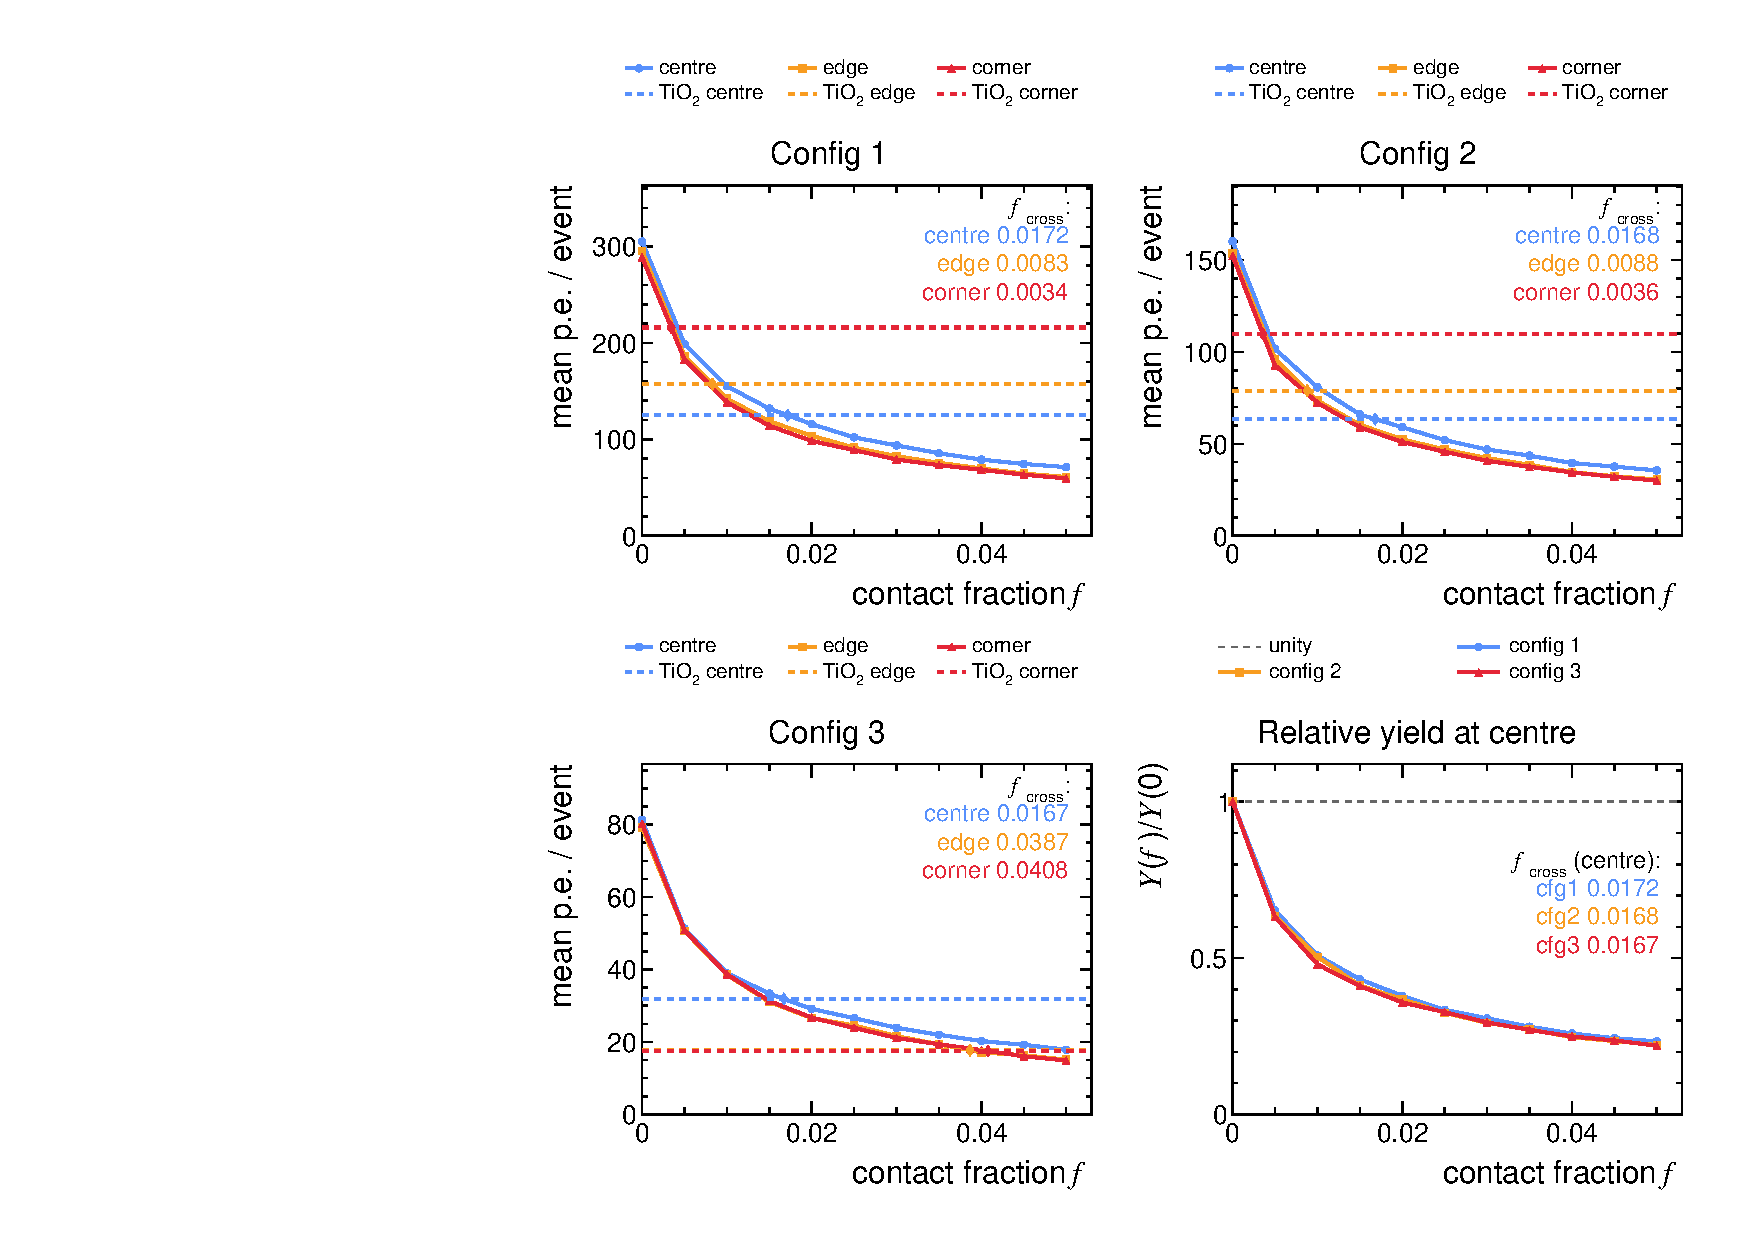
\includegraphics[width=\linewidth]{contact_scan.pdf}
  \end{column}
  \begin{column}{0.40\textwidth}
    {\small
    \begin{itemize}
      \item Clean gap ($f=0$) = near-lossless TIR guide: cfg-1 centre 305~pe.
      \item $f=0.01$ already halves light (155~pe); $f=0.03\to$ 94~pe.
      \item Centre crossing $f\approx0.017$ in all layouts; edge/corner 0.003--0.009 (cfg~1--2), $>0.03$ (cfg-3 far side).
      \item \textbf{No single $f$} matches every layout/position --- kept as systematic bracket, default stays $f=0$.
    \end{itemize}
    {\scriptsize Cf.\ report Fig.~17.}}
  \end{column}
  \end{columns}
\end{frame}

\begin{frame}{Al backing: grease vs air brackets the real foil}
  \begin{columns}[T]
  \begin{column}{0.58\textwidth}
    \centering
    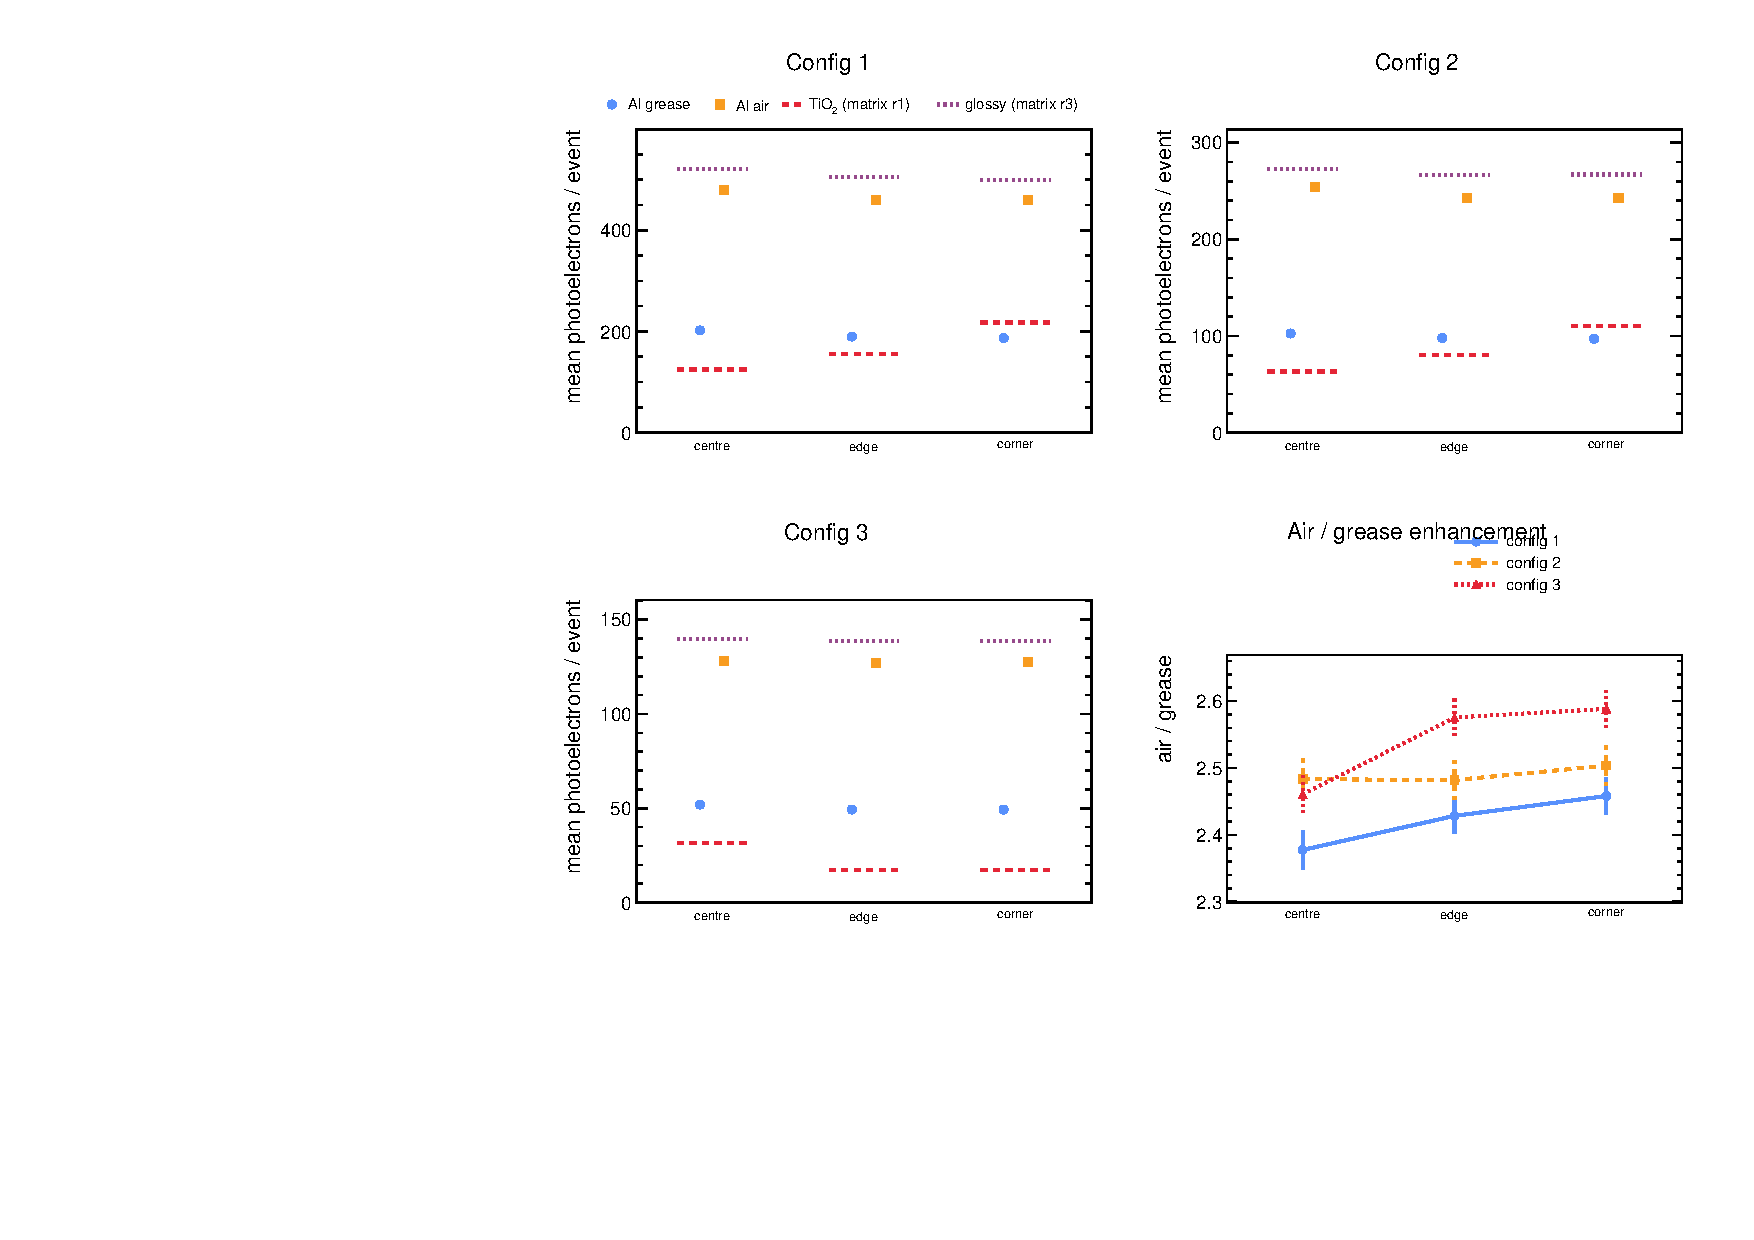
\includegraphics[width=\linewidth]{al_backing.pdf}
  \end{column}
  \begin{column}{0.40\textwidth}
    {\small
    \begin{itemize}
      \item Same $R(\lambda)$; only backing index changes $\theta_c$: grease \SI{67.5}{\degree} vs air \SI{39.3}{\degree}.
      \item Air raises Al 2.38--2.59$\times$: cfg-1 centre 202 $\to$ 480~pe.
      \item Air-backed Al $\approx$\SI{92}{\percent} of glossy --- recovers Rao's Al $\approx$ glossy.
      \item Production whole-slab used grease (conservative lower branch).
    \end{itemize}}
  \end{column}
  \end{columns}
\end{frame}

\begin{frame}{Full-plate maps: glossy/bare flat, TiO$_2$ graded}
  \begin{columns}[T]
  \begin{column}{0.50\textwidth}
    \centering
    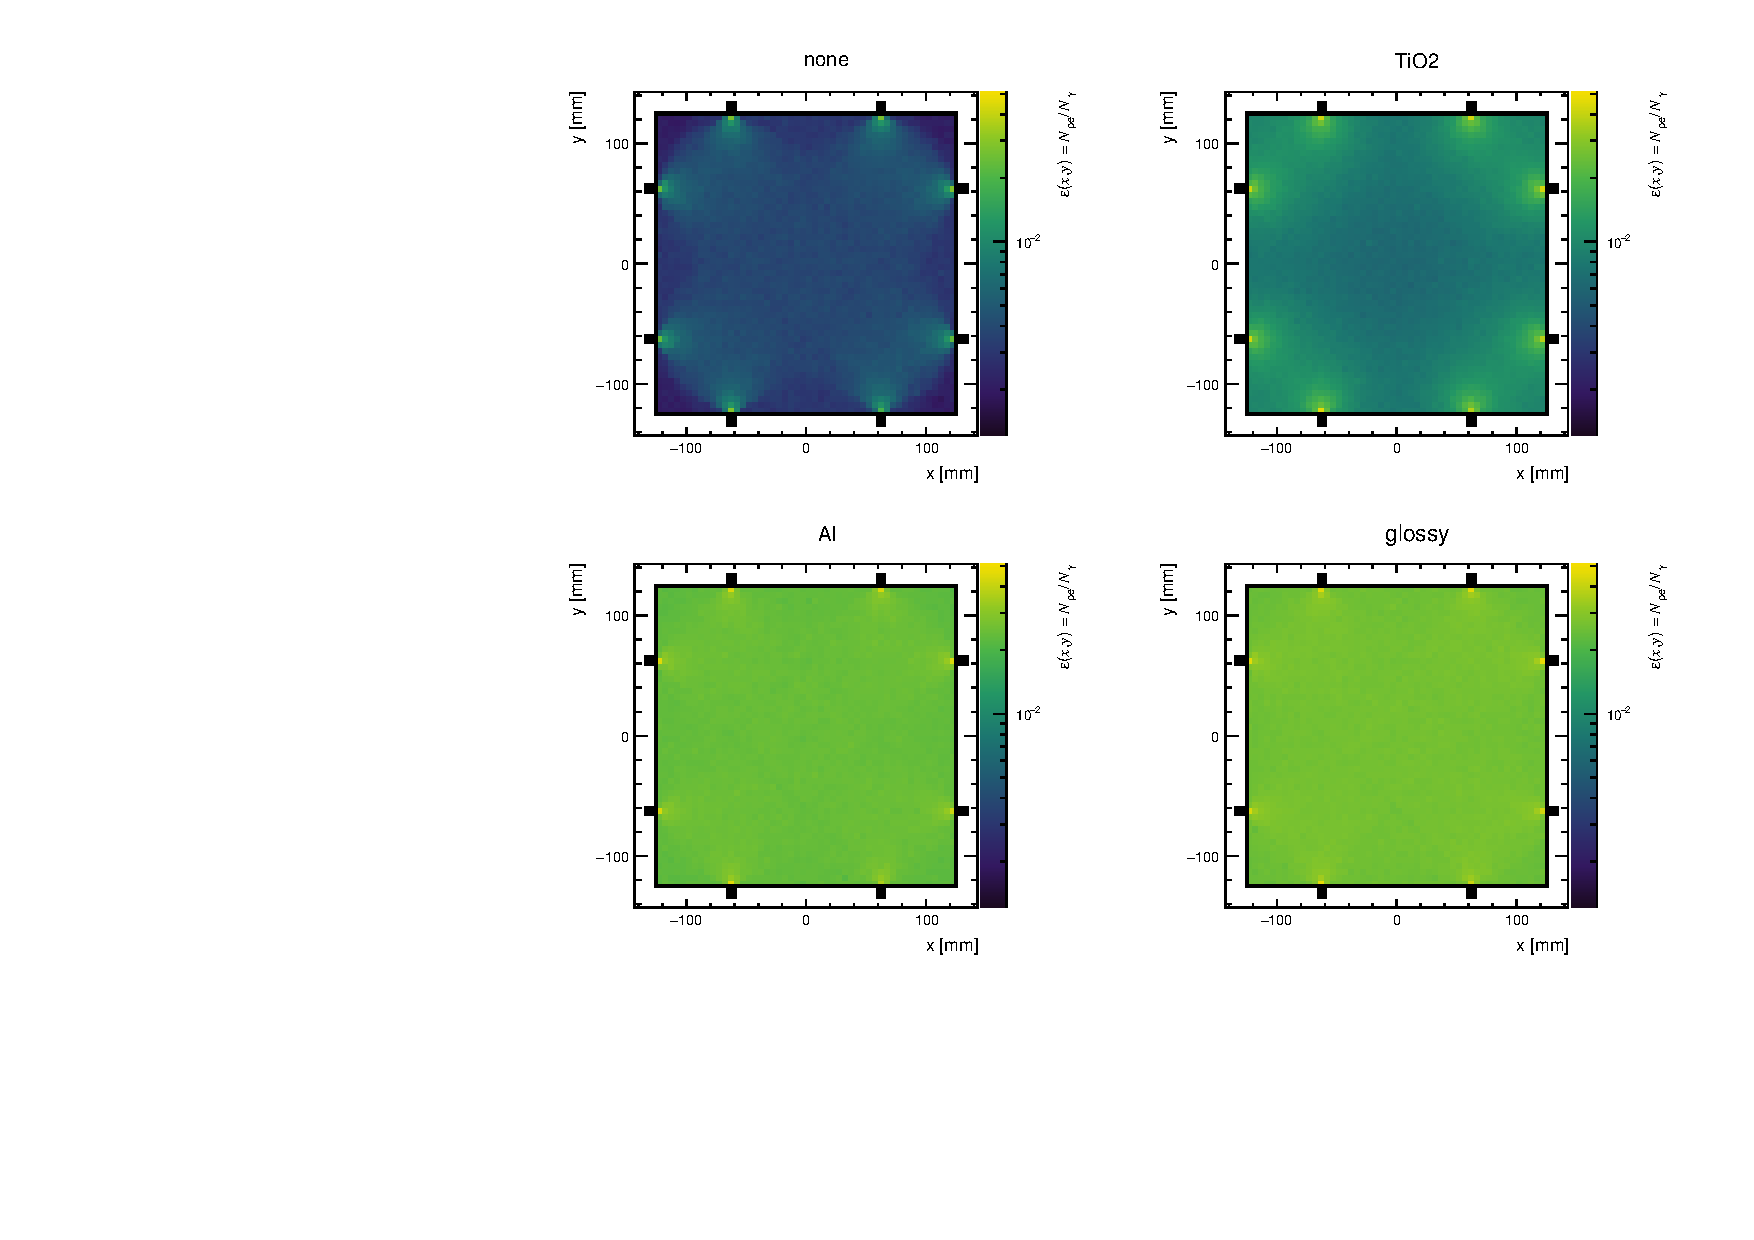
\includegraphics[width=\linewidth]{whole_slab_cfg1.pdf}\\
    {\scriptsize Cfg-1 maps, $5\times$\SI{5}{\milli\meter} cells, shared log-$z$. Bare/Al/glossy flat to $<$9\%; TiO$_2$ centre-dim (0.67\% vs 1.02\% outer, 1.51$\times$).}
  \end{column}
  \begin{column}{0.48\textwidth}
    \centering
    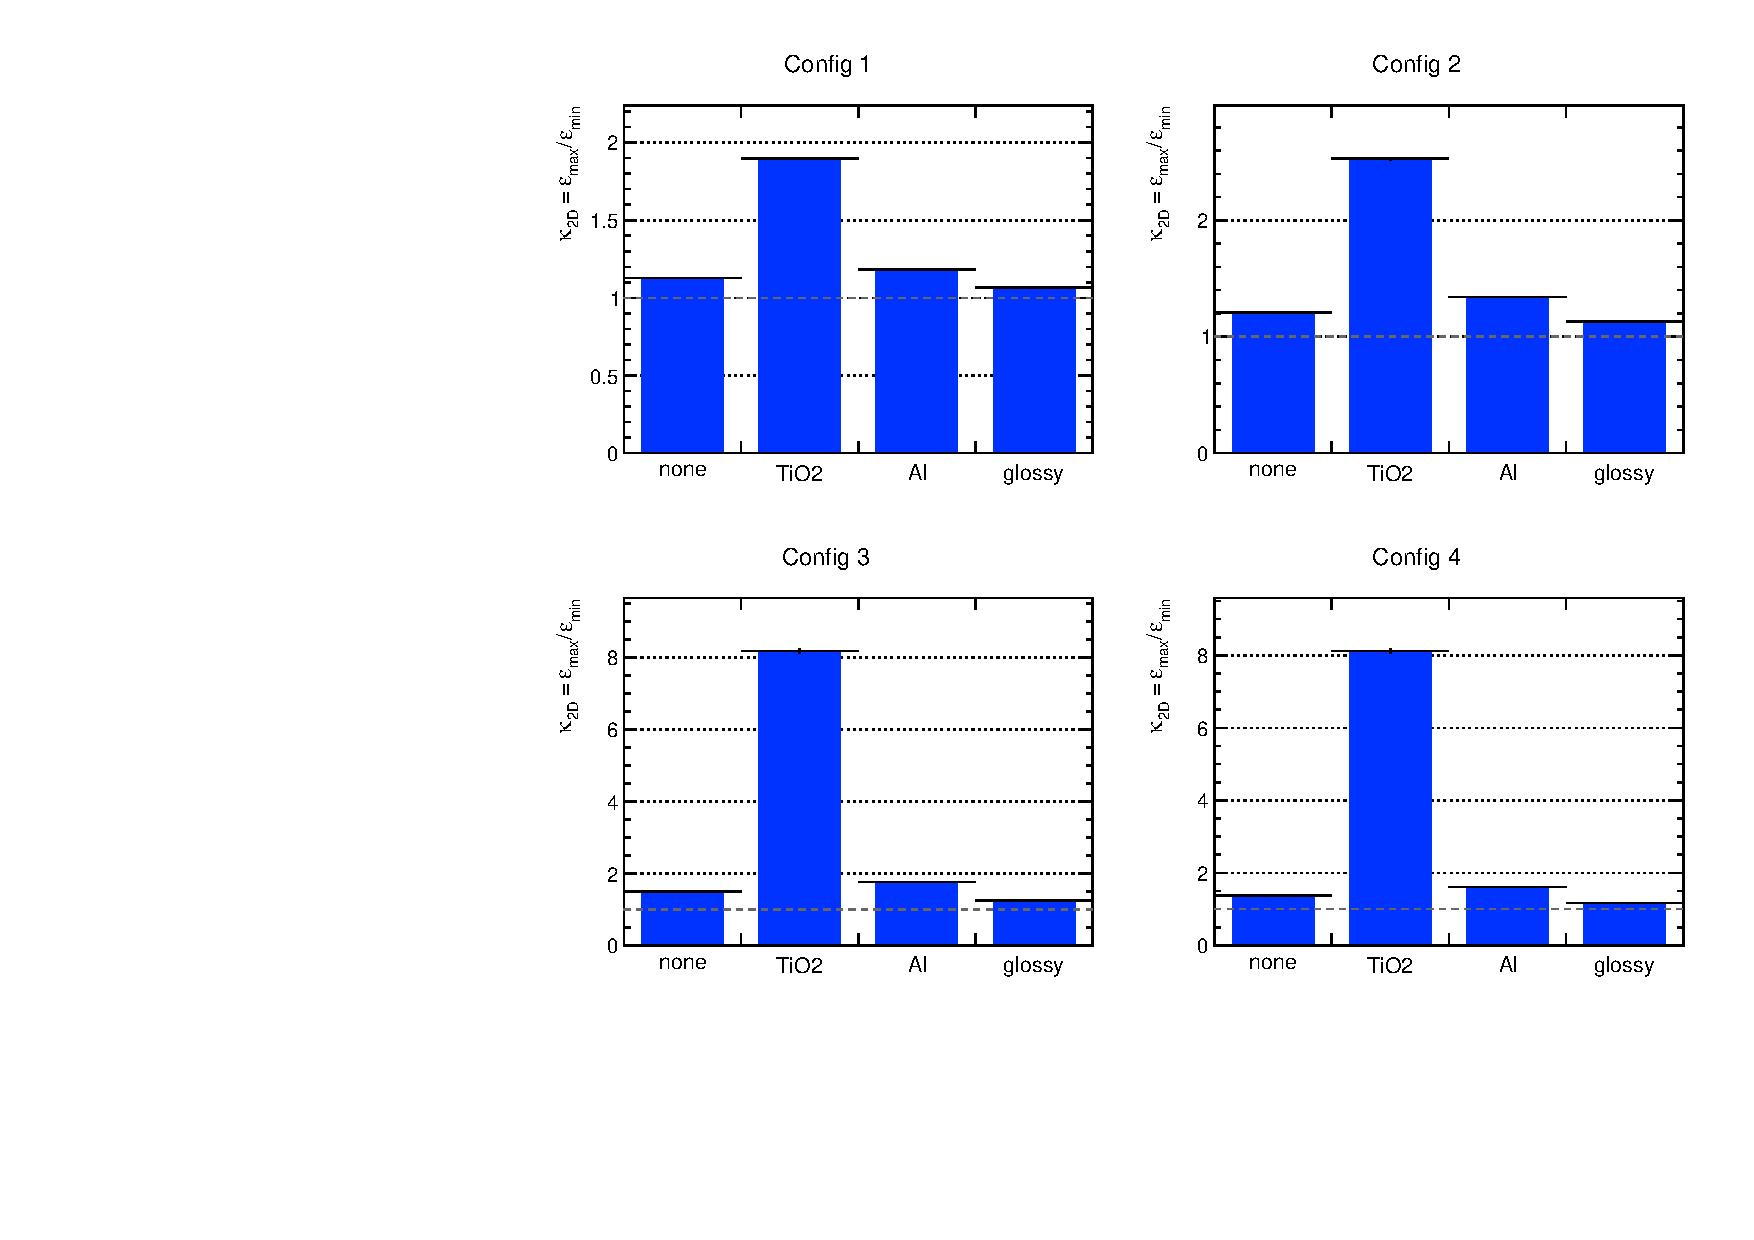
\includegraphics[width=0.85\linewidth]{fig_whole_contrast.pdf}\\
    {\scriptsize Contrast $\kappa_{\rm 2D}=$ max/min over \SI{50}{\milli\meter} cells. TiO$_2$ 1.9--8.2, bare 1.13--1.49, Al 1.18--1.77, glossy 1.07--1.25. Cf.\ report Figs.~19, 21--23.}
  \end{column}
  \end{columns}
\end{frame}

\begin{frame}{Pulses: persistence and average waveforms}
  \begin{columns}[T]
  \begin{column}{0.55\textwidth}
    \centering
    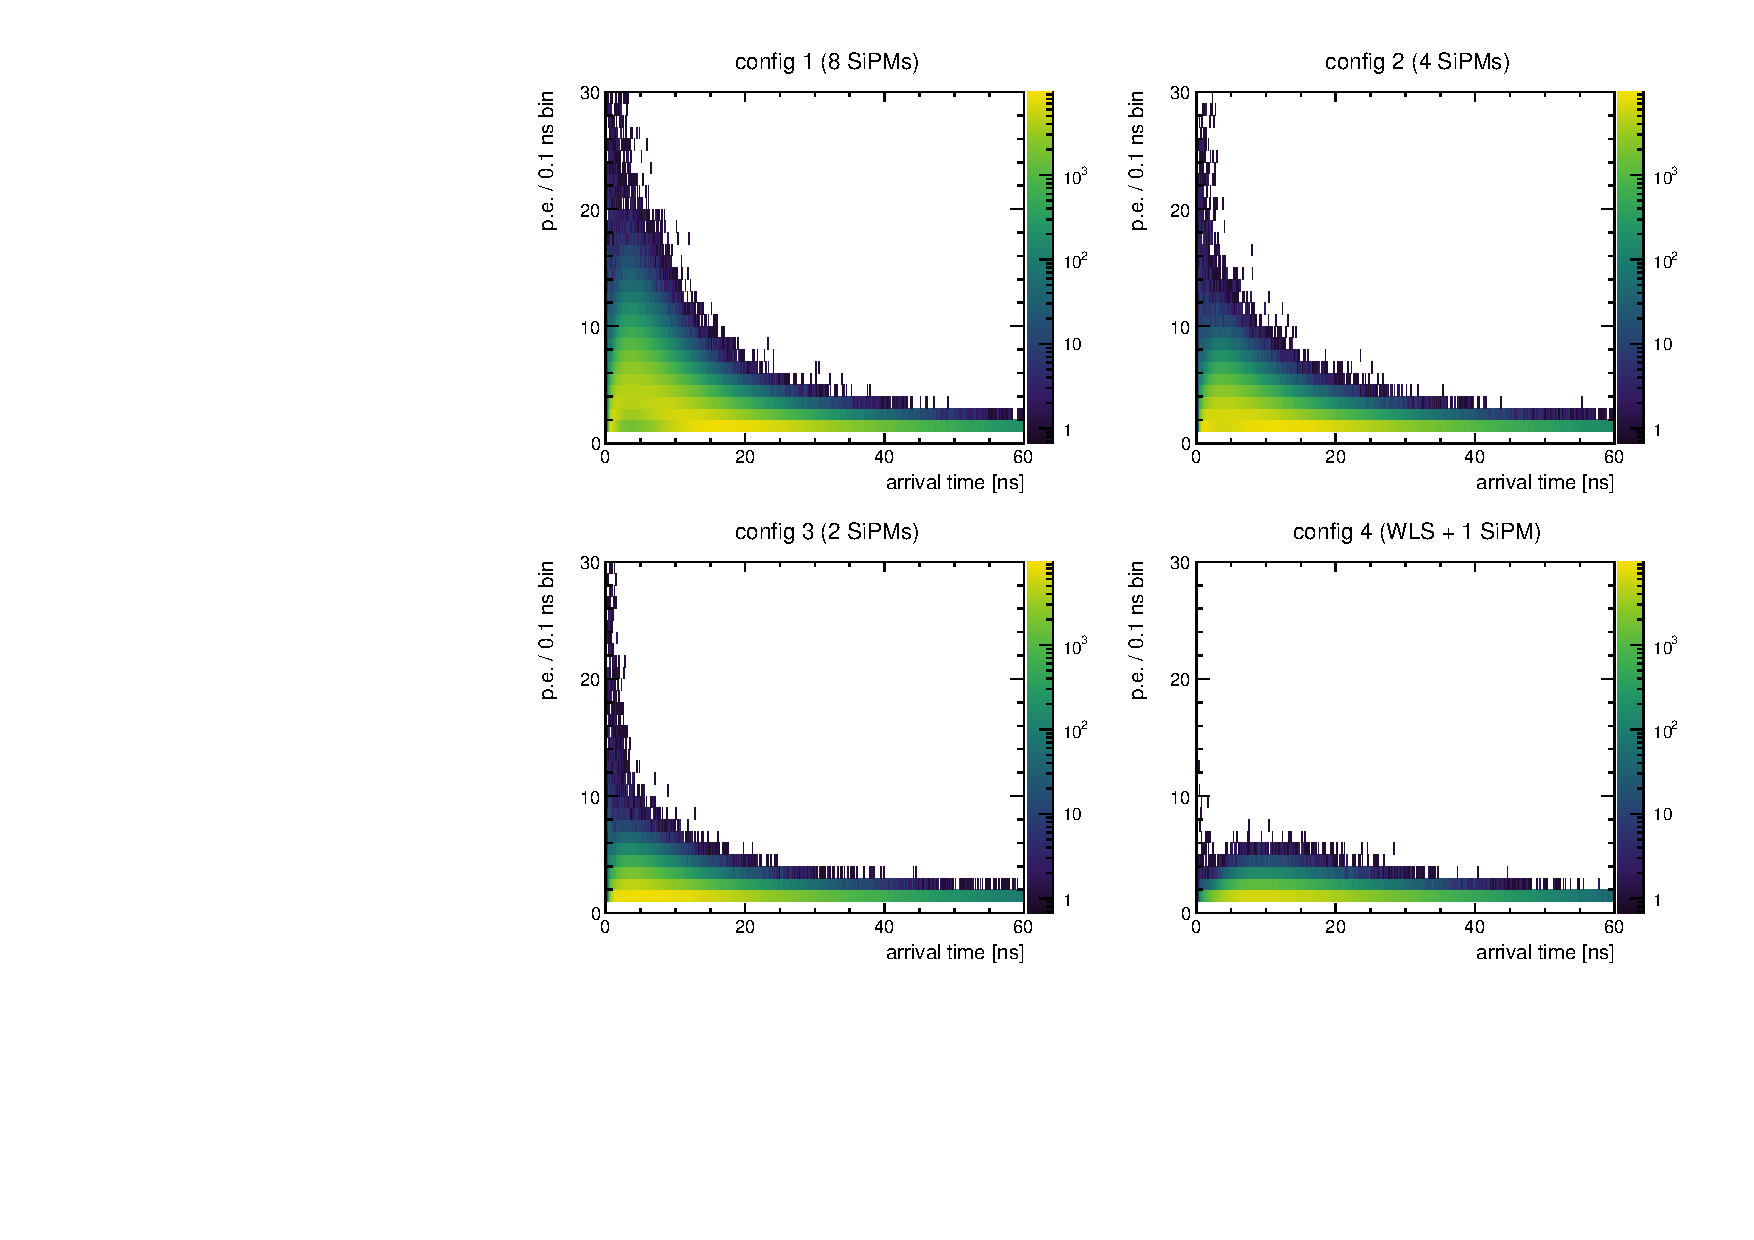
\includegraphics[width=\linewidth]{fig_persistence_grid.pdf}
  \end{column}
  \begin{column}{0.43\textwidth}
    \centering
    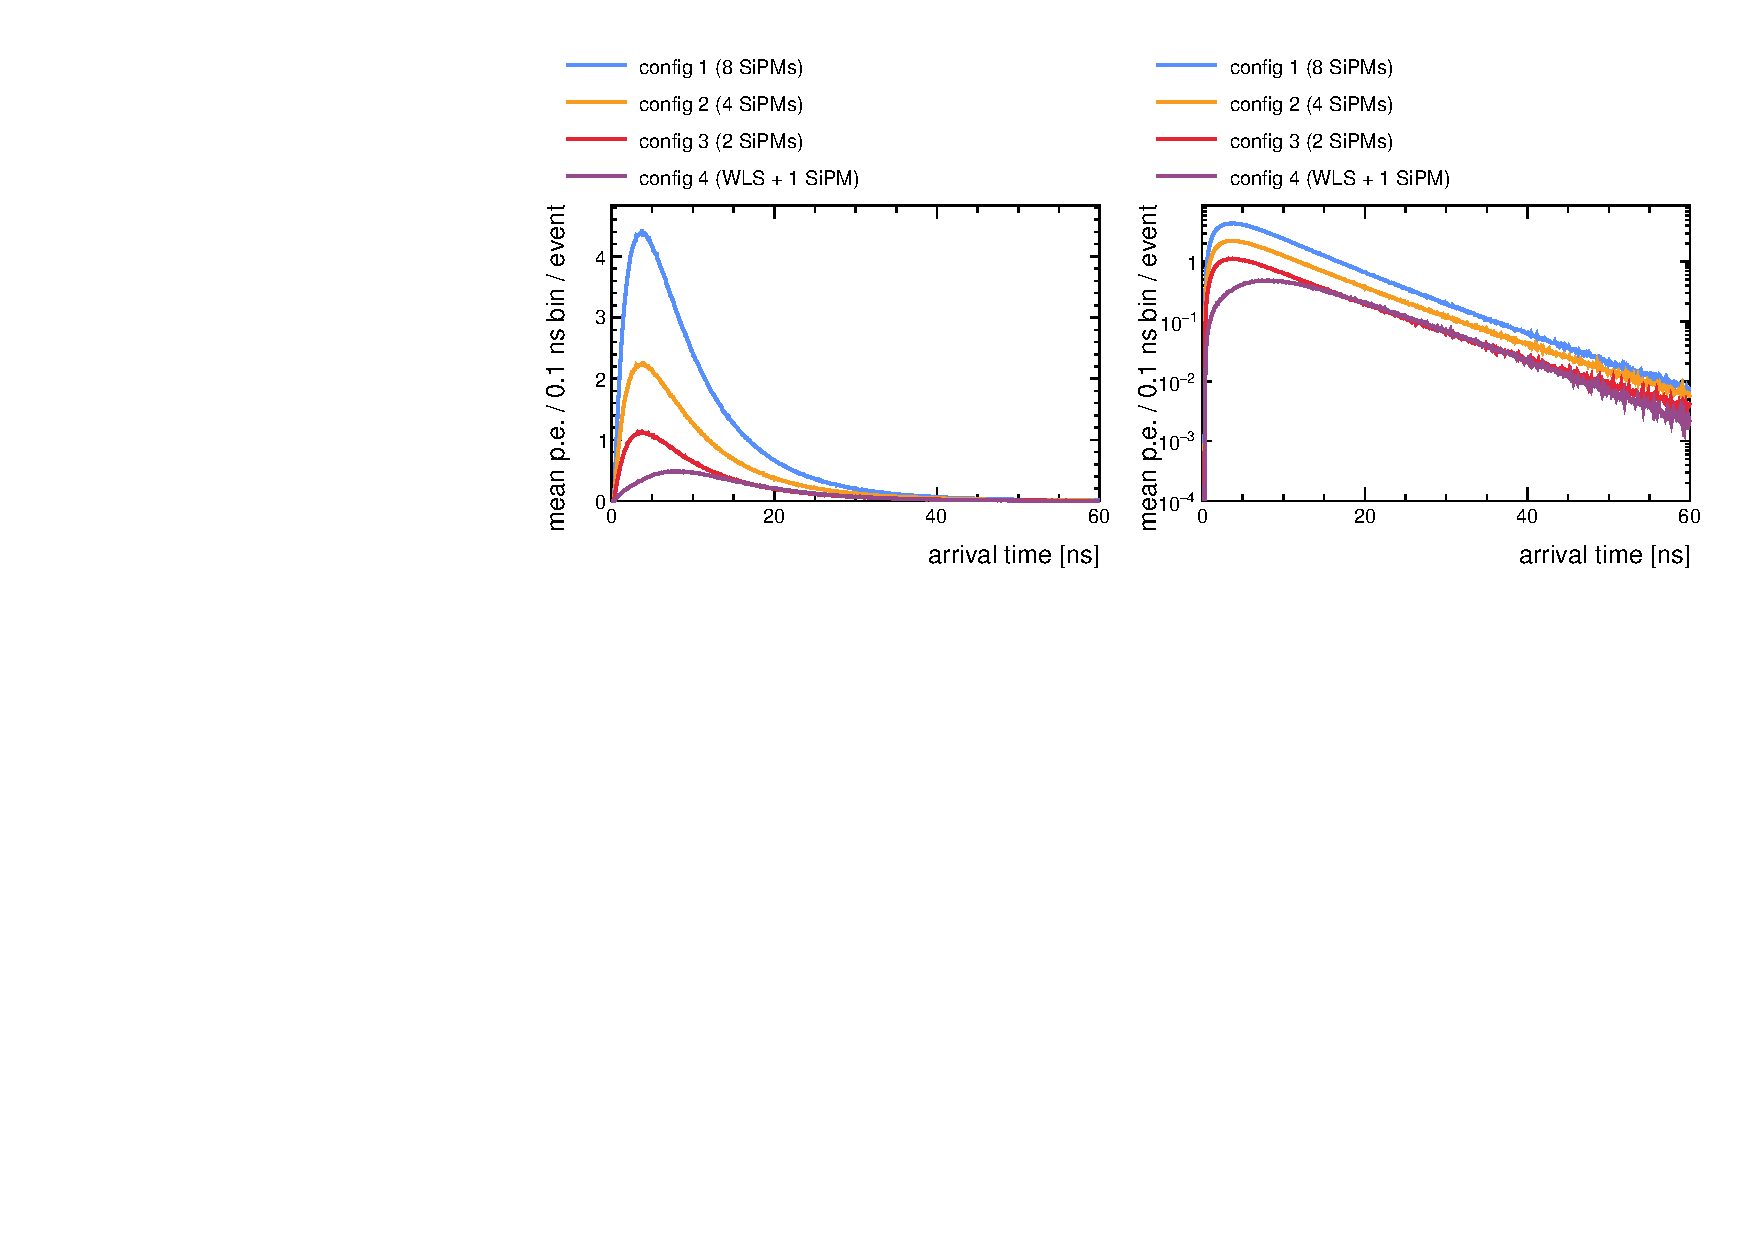
\includegraphics[width=\linewidth]{fig_avg_waveform.pdf}\\
    {\scriptsize Glossy, whole-plate. Modal arrival 3.8--4.0~ns (cfg~1--3) vs 9.25~ns (cfg-4); $\le$\SI{5}{\nano\meter} fractions 32/31/30/7\%; late ($>$\SI{20}{\nano\meter}) 11/12/13/25\%. Integrals: 520/274/140/68~pe. Cf.\ Figs.~29--30.}
  \end{column}
  \end{columns}
\end{frame}

\begin{frame}{Wavelength vs time + take-aways}
  \begin{columns}[T]
  \begin{column}{0.50\textwidth}
    \centering
    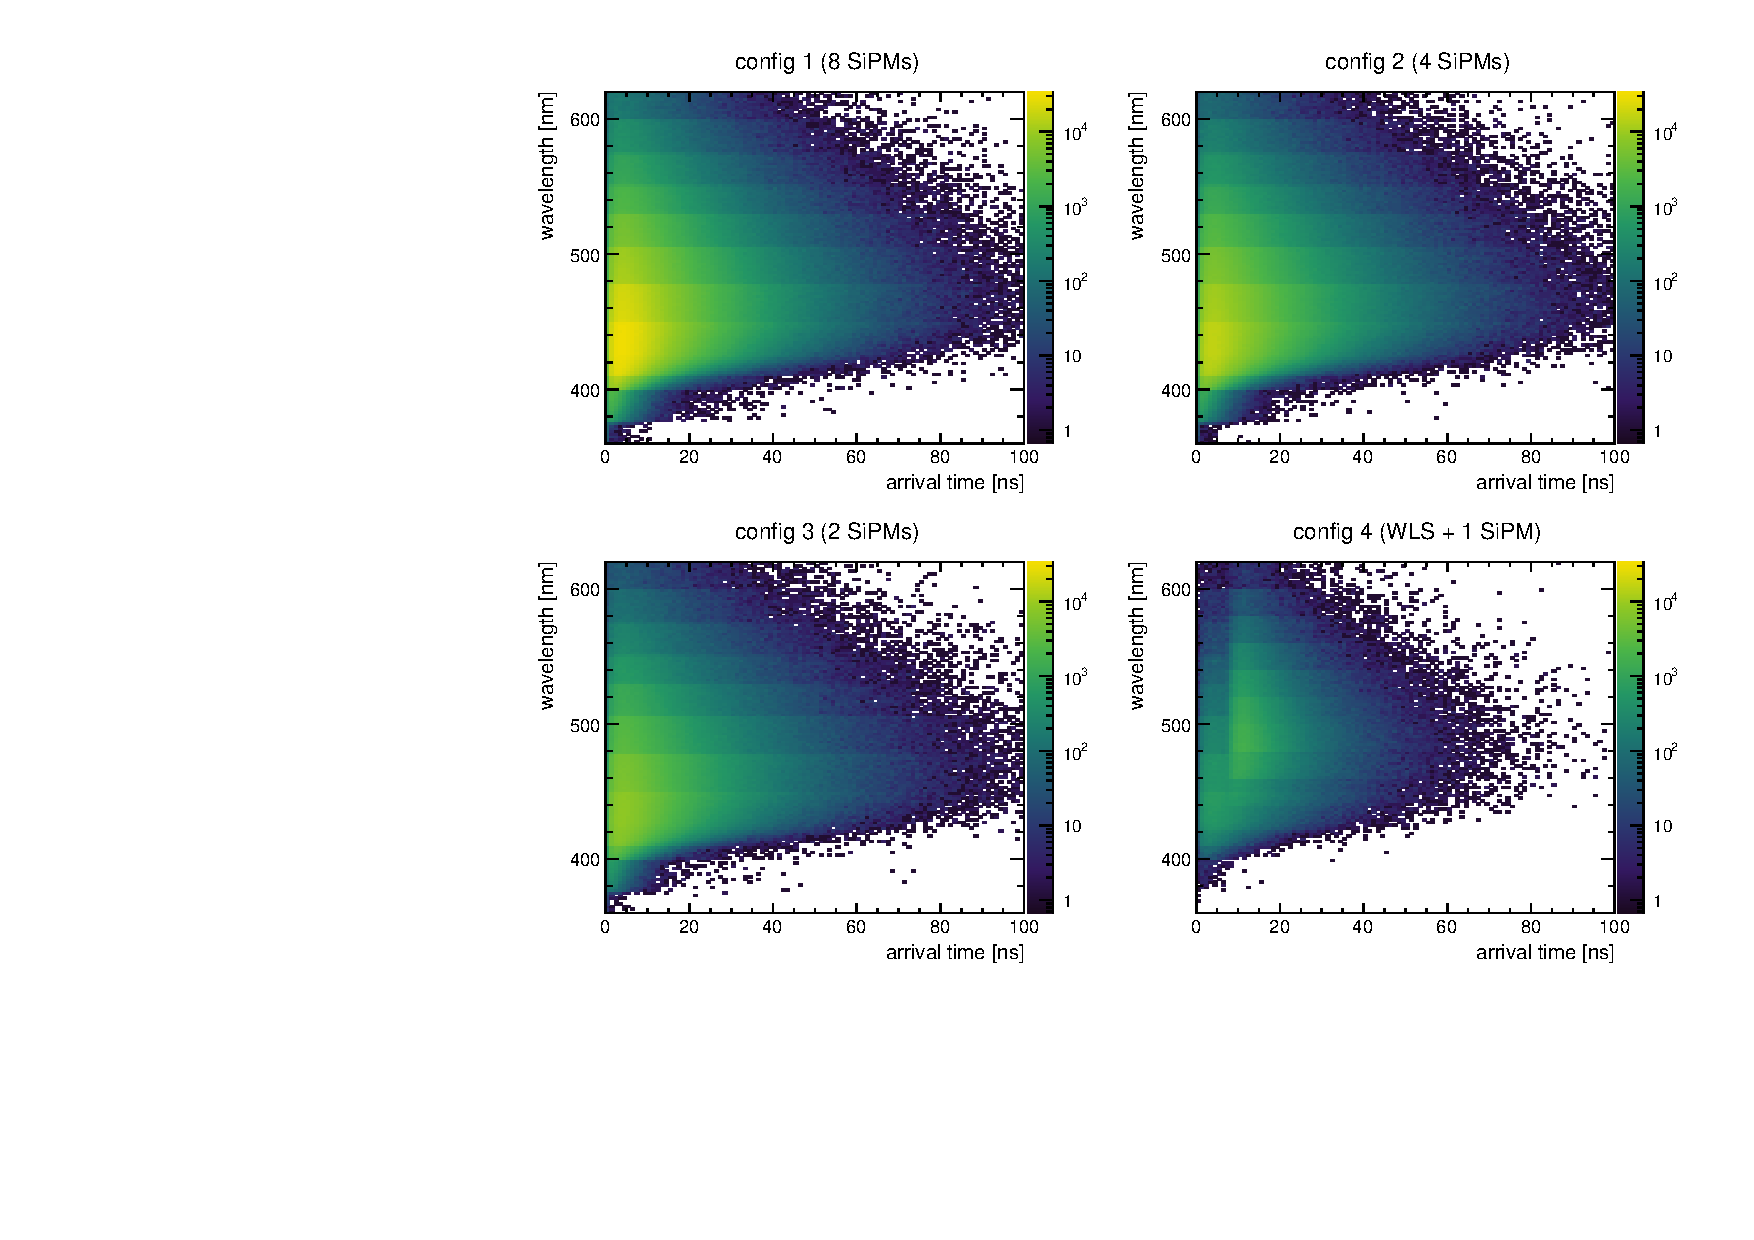
\includegraphics[width=\linewidth]{fig_wavelength_time_grid.pdf}\\
    {\scriptsize Mean $\lambda$: 450.9 $\to$ 467.7~nm (cfg~1--3), 498.9 $\to$ 511.3~nm (cfg-4): late light reddens by self-absorption. Cf.\ Fig.~31.}
  \end{column}
  \begin{column}{0.48\textwidth}
    {\small
    \textbf{What we reproduce}
    \begin{itemize}
      \item Glossy brightest + most uniform in every layout; TiO$_2$ weakest (cfgs~1--3) and most position-dependent.
    \end{itemize}
    \textbf{What we don't}
    \begin{itemize}
      \item Bare is 2nd-brightest (TIR guide), not weakest; needs $f\approx0.017$ contact to fall below TiO$_2$.
      \item TiO$_2$ corner-highest in cfg~1--2, vs paper corner-lowest.
      \item Cfg-4 $\approx$67~pe (glossy centre) $<$ cfg-3, vs paper cfg-4 $>$ cfg-3 (different normalisation/gain noted).
    \end{itemize}
    \textbf{Bottom line:} wrapper sets ordering, layout sets scale; $f$ and Al-backing brackets quantify the systematics.}
  \end{column}
  \end{columns}
\end{frame}

\end{document}
